% ============================================================
% HSBI Beamer — ISLP Lecture Series — IMPROVED EDITION
% Advanced Module A4: GLMs and Splines
% ============================================================
\documentclass[aspectratio=169,11pt]{beamer}
\usepackage[utf8]{inputenc}\usepackage[T1]{fontenc}\usepackage[english]{babel}
\usepackage{graphicx}\usepackage{booktabs}\usepackage{amsmath,amssymb,amsfonts}
\usepackage{mathtools}\usepackage{hyperref}\usepackage{xcolor}
\usepackage{verbatim}\usepackage{alltt}
\usepackage{tikz}\usetikzlibrary{calc,arrows.meta,positioning,shapes}
\usepackage{tcolorbox}\tcbuselibrary{skins}

\usetheme{Madrid}\usecolortheme{default}
\setbeamertemplate{navigation symbols}{}
\setbeamertemplate{footline}[frame number]
\setbeamertemplate{blocks}[rounded][shadow=false]
\setbeamertemplate{headline}{%
  \leavevmode\hbox{%
    \begin{beamercolorbox}[wd=\paperwidth,ht=2.2ex,dp=0.9ex]{section in head/foot}%
      {\fontsize{4.6}{5.2}\selectfont%
       \insertsectionnavigationhorizontal{\paperwidth}{}{\hskip0pt plus1filll}}%
    \end{beamercolorbox}}%
}
\setbeamerfont{section in head/foot}{size=\tiny}
\setbeamerfont{palette primary}{size=\tiny}
\setbeamerfont{palette tertiary}{size=\tiny}
\setbeamerfont{section in toc}{size=\footnotesize}

\usepackage{listings}
\definecolor{pyKw}{RGB}{0,0,180}\definecolor{pyStr}{RGB}{20,120,40}
\definecolor{pyCom}{RGB}{120,120,120}\definecolor{accent}{RGB}{38,70,140}
\lstdefinestyle{Pystyle}{language=Python,basicstyle=\ttfamily\footnotesize,
  keywordstyle=\color{pyKw}\bfseries,commentstyle=\color{pyCom}\itshape,
  stringstyle=\color{pyStr},showstringspaces=false,upquote=true,
  columns=fullflexible,breaklines=true,literate={~}{{$\sim$}}1}
\lstset{style=Pystyle}

% Tighter TOC spacing (place AFTER \lstset, BEFORE \AtBeginSection)
\usepackage{etoolbox}
\makeatletter
\patchcmd{\beamer@sectionintoc}{\vskip1.5em}{\vskip.6em}{\typeout{TOCPATCH-OK}}{\typeout{TOCPATCH-FAIL}}
\makeatother

\AtBeginSection[]{\begin{frame}{Outline}\footnotesize
  \tableofcontents[currentsection,sectionstyle=show/shaded,subsectionstyle=show/show/hide]
\end{frame}}

\newcommand{\islpsource}[1]{%
  \vfill\hfill{\tiny\itshape\color{gray}Source: #1 \textemdash{} ISLP, James et al.\ (2023).}\par
}

\newtcolorbox{takeaway}[1][Takeaway]{enhanced,colback=green!4,colframe=green!50!black,
  boxrule=0pt,leftrule=2.5pt,arc=2pt,fonttitle=\bfseries,title=#1,
  left=2mm,right=2mm,top=1mm,bottom=1mm}
\newtcolorbox{numexample}[1][Worked example]{enhanced,colback=orange!4,colframe=orange!70!black,
  boxrule=0pt,leftrule=2.5pt,arc=2pt,fonttitle=\bfseries,title=#1,
  left=2mm,right=2mm,top=1mm,bottom=1mm}
\newtcolorbox{readme}[1][How to read this]{enhanced,colback=blue!4,colframe=accent,
  boxrule=0pt,leftrule=2.5pt,arc=2pt,fonttitle=\bfseries,title=#1,
  left=2mm,right=2mm,top=1mm,bottom=1mm}

\title{Quantitative Research Methods}
\subtitle{GLMs and Splines\\[2pt]{\small Advanced module A4 --- optional self-study}}
\author{Prof.\ Dr.\ Christoph Weisser}\institute{HSBI}
\date{Summer Semester 2026}\graphicspath{{images/}}

\newtcolorbox{exercise}[1][Exercise]{enhanced, fontupper=\footnotesize, colback=purple!4, colframe=purple!55!black, boxrule=0pt, leftrule=2.5pt, arc=2pt, fonttitle=\bfseries, title=#1, left=2mm, right=2mm, top=1mm, bottom=1mm}
\newtcolorbox{solutionbox}[1][Solution]{enhanced, fontupper=\footnotesize, colback=teal!5, colframe=teal!55!black, boxrule=0pt, leftrule=2.5pt, arc=2pt, fonttitle=\bfseries, title=#1, left=2mm, right=2mm, top=1mm, bottom=1mm}
\newtcolorbox{longexercise}[1][Extended exercise (15 min)]{enhanced, fontupper=\footnotesize, colback=violet!6, colframe=violet!55!black, boxrule=0pt, leftrule=3pt, arc=2pt, fonttitle=\bfseries, title=#1, left=2mm, right=2mm, top=1mm, bottom=1mm}

% Reclaim ~2pt of body height (custom nav headline makes full slides tip over by ~1.83pt)
\addtobeamertemplate{frametitle}{}{\vspace{-2pt}}

\newtcolorbox{labnote}[1][Run this live in the lab notebook]{enhanced, fontupper=\footnotesize, colback=cyan!7, colframe=cyan!45!black, boxrule=0pt, leftrule=3pt, arc=2pt, fonttitle=\bfseries, title=#1, left=2mm, right=2mm, top=1mm, bottom=1mm}

% Industry application callout box --- slate grey, for real business/industry use
\definecolor{industryC}{RGB}{88,98,116}
\newtcolorbox{industry}[1][In industry]{enhanced, fontupper=\footnotesize, colback=industryC!7, colframe=industryC, boxrule=0pt, leftrule=3pt, arc=2pt, fonttitle=\bfseries, title={In industry --- #1}, left=2mm, right=2mm, top=1mm, bottom=1mm}

% Common-mistake callout --- crimson, for the error to pre-empt
\newtcolorbox{mistake}[1][Common mistake]{enhanced, fontupper=\footnotesize, colback=red!4, colframe=red!60!black, boxrule=0pt, leftrule=3pt, arc=2pt, fonttitle=\bfseries, title=#1, left=2mm, right=2mm, top=1mm, bottom=1mm}

\begin{document}
\begin{frame}[plain]\titlepage\end{frame}

\begin{frame}{Where this module fits}
  \footnotesize
  This is an \textbf{optional advanced module}: nothing in it is required for the exam,
  and everything in it deepens material you have already met.
  \begin{center}
  \begin{tabular}{@{}c l l@{}}
    & \textbf{Course chapter} & \textbf{What this module adds} \\
    \midrule
    & Ch.\ 3 --- Linear regression & \ldots{}becomes the \emph{Gaussian corner} of one big family \\
    & Ch.\ 4 --- Classification & \ldots{}logistic and Poisson regression re-derived as GLMs \\
    & Ch.\ 5 --- Resampling & \ldots{}CV and GCV choose the spline penalty $\lambda$ \\
    & Ch.\ 6 --- Model selection & \ldots{}deviance, likelihood-ratio tests and AIC for GLMs \\
    $\blacktriangleright$ & \textbf{Ch.\ 7 --- Splines and GAMs} & \textbf{\ldots{}penalized splines, and GAMs for count data} \\
  \end{tabular}
  \end{center}
  \vspace{2pt}
  \begin{takeaway}[One sentence]
    Chapter 4's likelihood view and Chapter 7's smooth curves are two halves of the same
    machine --- this module assembles it: \textbf{exponential family $\to$ GLM $\to$
    penalized spline $\to$ GAM for counts}, all on one real dataset (\texttt{Bikeshare}).
  \end{takeaway}
\end{frame}

\begin{frame}{Contents}\small\tableofcontents[hideallsubsections]
  \vfill
  {\tiny Optional and advanced material is collected in the \textbf{appendix} at the end of the deck.}
\end{frame}

\begin{frame}{Notation in this module}
  \footnotesize
  \begin{center}
  \begin{tabular}{@{}ll@{}}
    \toprule
    \textbf{Symbol} & \textbf{Meaning} \\
    \midrule
    $Y_i$, $y_i$ & response (here: hourly count of bikers); its observed value \\
    $\mu_i = E[Y_i]$ & mean of the response for observation $i$ \\
    $\theta$, $\phi$ & canonical (natural) parameter; dispersion parameter \\
    $b(\theta)$, $a(\phi)$, $c(y,\phi)$ & the three building blocks of an exponential-family density \\
    $V(\mu)$ & variance function: $\operatorname{Var}(Y) = a(\phi)\,V(\mu)$ \\
    $\eta_i = x_i^{\top}\beta$ & linear predictor \\
    $g(\cdot)$ & link function, $g(\mu_i)=\eta_i$; canonical link $g = (b')^{-1}$ \\
    $D$, $D_0$ & residual deviance; null deviance (intercept-only model) \\
    $\hat\varphi$ & Pearson estimate of the dispersion (quasi-Poisson) \\
    $\alpha$ & negative-binomial overdispersion: $\operatorname{Var}=\mu+\alpha\mu^2$ \\
    $B_j(x)$, $\beta_j$ & $j$-th B-spline basis function; its coefficient \\
    $\lambda$, $S$ & smoothing penalty weight; penalty matrix, $\int f''(t)^2 dt=\beta^\top S\beta$ \\
    edf & effective degrees of freedom, $\operatorname{tr}\{H(\lambda)\}$ \\
    $f_j(\cdot)$ & smooth partial effect of predictor $j$ in a GAM \\
    \bottomrule
  \end{tabular}
  \end{center}
\end{frame}

\begin{frame}{Sources and references}
  \begin{block}{Primary textbook}
    James, G., Witten, D., Hastie, T., Tibshirani, R., \& Taylor, J.\ (2023).
    \emph{An Introduction to Statistical Learning, with Applications in
    Python.} Springer. --- Sections 4.6 (Poisson regression) and Chapter 7 (splines, GAMs).
  \end{block}
  \begin{block}{Going deeper (optional)}
    McCullagh, P.\ \& Nelder, J.\ (1989). \emph{Generalized Linear Models}, 2nd ed., Chapman \& Hall.\\
    Wood, S.\ (2017). \emph{Generalized Additive Models: An Introduction with R}, 2nd ed., CRC Press.\\
    Eilers, P.\ \& Marx, B.\ (1996). Flexible smoothing with B-splines and penalties. \emph{Statistical Science}, 11(2).
  \end{block}
\end{frame}

\begin{frame}{Learning objectives}
  By the end of this module you will be able to:
  \begin{itemize}
    \item \textbf{Explain} the exponential family and derive a member's mean and variance from $b(\theta)$.
    \item \textbf{Specify} a GLM --- random component, linear predictor, link --- for a given data type.
    \item \textbf{Interpret} Poisson coefficients as rate ratios, and \textbf{use} offsets for exposure.
    \item \textbf{Test} nested GLMs with deviance and likelihood-ratio tests, and \textbf{compare} models with AIC.
    \item \textbf{Diagnose} overdispersion and \textbf{choose} between quasi-Poisson and negative binomial.
    \item \textbf{Tune} a penalized spline via GCV or CV and \textbf{read} its effective degrees of freedom.
    \item \textbf{Fit} and \textbf{interpret} a penalized-spline GAM for counts with \texttt{statsmodels}.
  \end{itemize}
\end{frame}

\begin{frame}{Roadmap of this module}
  \begin{takeaway}[From a broken linear model to a GAM for counts]
    \begin{enumerate}
      \item Why the linear model fails on \texttt{Bikeshare} counts.
      \item The exponential family: one density form behind Chs.\ 3 and 4.
      \item GLM anatomy: random component + linear predictor + link; Poisson regression, offsets.
      \item Inference: deviance, likelihood-ratio tests, AIC.
      \item Overdispersion: quasi-Poisson and the negative binomial.
      \item Splines deepened: B-spline bases, roughness penalties, effective df, GCV.
      \item The meeting point: penalized-spline GAMs for counts.
    \end{enumerate}
  \end{takeaway}
\end{frame}

\begin{frame}{Where this module is used in industry}
  \scriptsize
  \begin{center}
  \begin{tabular}{@{}p{2.6cm}p{5.2cm}p{4.6cm}@{}}
    \toprule
    \textbf{Sector} & \textbf{Concrete application} & \textbf{Which decision it drives} \\
    \midrule
    Insurance & Claim \emph{frequency} as a Poisson/NB GLM with exposure offsets; age curves as GAM smooths & The premium each tariff cell pays \\
    Retail, e-commerce & Daily demand counts per SKU and store, weather and calendar smooths & Ordering, staffing and markdowns \\
    Energy & Load forecasting with GAMs: smooth effects of temperature and time of day & How much generation to schedule \\
    Public health & Case and admission counts vs exposure population & Staffing, stockpiles, early warnings \\
    Banking & Default (yes/no) as a logistic GLM --- the same machinery & Approve or decline; capital held \\
    Mobility platforms & Hourly ride counts vs hour, weather, events (this module's dataset) & Fleet rebalancing and surge staffing \\
    \bottomrule
  \end{tabular}
  \end{center}
  \begin{industry}[The common thread]
    Whenever the response is a \textbf{count} or a \textbf{rate}, industry reaches for exactly
    this stack: GLM for interpretability and valid uncertainty, smooth terms for the
    shapes no one wants to guess, offsets for unequal exposure.
  \end{industry}
\end{frame}

\begin{frame}{Industry case in depth: pricing motor insurance}
  \footnotesize
  \begin{industry}[Claim frequency at a motor insurer]
    A pricing team models the \textbf{number of claims} per policy-year for millions of
    policies. Policies are observed for unequal durations --- three months here, a full
    year there --- so the model is a Poisson GLM for the claim \emph{rate} with
    $\log(\text{exposure})$ as an \textbf{offset}. Tariff factors (region, vehicle class,
    bonus--malus) enter as dummies; \textbf{driver age} enters as a penalized-spline smooth,
    because its effect is famously U-shaped and no polynomial degree is defensible to a regulator.
  \end{industry}
  \begin{readme}[Why the family matters commercially]
    The premium is roughly $\text{frequency}\times\text{severity}$. If the frequency model
    ignores \textbf{overdispersion}, its standard errors are far too small: tariff cells look
    ``significantly'' different when they are not, and the tariff fragments into noise.
    Actuarial practice therefore fits quasi-Poisson or negative binomial by default.
  \end{readme}
  \begin{takeaway}
    Every ingredient of this module --- log link, rate ratios, offsets, overdispersion,
    spline smooths, edf --- appears in one production pricing model.
  \end{takeaway}
\end{frame}

% ============================================================
\section{Counts Break the LM}
% ============================================================

\begin{frame}{The \texttt{Bikeshare} data: $8\,645$ hours of counts}
  \footnotesize
  Hourly bike rentals in Washington DC (ISLP): response \texttt{bikers}, the number of
  riders in that hour.
  \begin{center}
  \begin{tabular}{@{}llll@{}}
    \toprule
    \textbf{Variable} & \textbf{Type} & \textbf{Range / levels} & \textbf{Role} \\
    \midrule
    \texttt{bikers} & count & 1 to 651 & response \\
    \texttt{hr} & hour of day & 0--23 & 23 dummies (or a smooth) \\
    \texttt{temp} & normalised temperature & 0.02--1 ($1\approx 41^{\circ}$C) & numeric \\
    \texttt{workingday} & binary & 0/1 & dummy \\
    \texttt{weathersit} & categorical & clear / cloudy-misty / light rain / heavy rain & 3 dummies \\
    \bottomrule
  \end{tabular}
  \end{center}
  \begin{numexample}[The response at a glance]
    $n=8\,645$ hours; mean $\bar y = 143.8$ bikers, variance $s^2 = 17\,902$ ---
    the variance is about $\mathbf{124\times}$ the mean. Weather levels are very
    unbalanced: clear $5\,645$, cloudy/misty $2\,218$, light rain/snow $781$,
    heavy rain/snow \textbf{a single hour}.
  \end{numexample}
  \begin{takeaway}
    A count response lives on $\{0,1,2,\dots\}$ and its spread grows with its level.
    Keep both facts in mind --- the linear model respects neither.
  \end{takeaway}
\end{frame}

\begin{frame}{Fit the Chapter-3 linear model \ldots{}and watch it fail}
  \begin{center}
    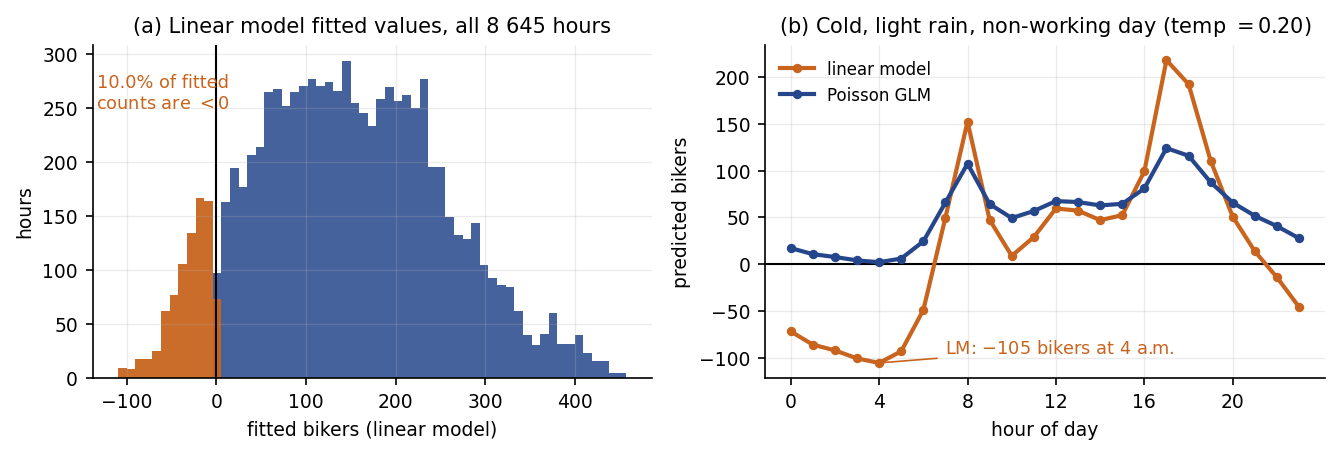
\includegraphics[width=0.9\textwidth,height=0.52\textheight,keepaspectratio]{adv04_lm_vs_glm.png}
  \end{center}
  \begin{takeaway}
    \footnotesize
    OLS on \texttt{bikers $\sim$ hr + temp + workingday + weathersit}: \textbf{10.0\%}
    of fitted values ($861$ of $8\,645$ hours) are \emph{negative}; on a cold rainy
    night it predicts $\mathbf{-105}$ riders at 4\,a.m.\ --- the Poisson GLM (right)
    predicts $2.2$: small, positive, sensible.
  \end{takeaway}
\end{frame}

\begin{frame}{Two failures, one diagnosis}
  \footnotesize
  \begin{readme}[What exactly is wrong with the Gaussian linear model here?]
    Model under indictment: $Y = x^{\top}\beta + \varepsilon$,
    $\varepsilon\sim N(0,\sigma^2)$.
    \begin{enumerate}
      \item \textbf{Wrong support.} A Gaussian mean can be negative; a count cannot.
            The $10.0\%$ negative predictions are the model doing what it was told.
      \item \textbf{Wrong variance.} Constant $\sigma^2$ --- but quiet 4\,a.m.\ hours
            vary by a few riders, busy 5\,p.m.\ hours by hundreds: variance
            \emph{grows with the mean}.
    \end{enumerate}
  \end{readme}
  \begin{takeaway}[What we need instead]
    A model whose \textbf{mean respects the data type}, whose \textbf{variance is tied
    to the mean}, and which keeps a \textbf{linear predictor} $x^{\top}\beta$ we know
    how to estimate and interpret. That is precisely a \emph{generalized linear model}.
  \end{takeaway}
  \begin{industry}[Mobility platforms: why negative forecasts hurt]
    A fleet-rebalancing optimiser fed ``$-105$ rides expected'' will happily truck
    bikes \emph{away} from a station that will see riders at dawn.
  \end{industry}
\end{frame}

% ------------------------------------------------------------
\begin{frame}{Exercise A4.1 --- Choosing the random component [Concept]}
\begin{exercise}
  \begin{enumerate}
    \item Name the \textbf{two} distinct failures of the Gaussian linear model on hourly
          bike counts, and say which \emph{observable symptom} each produces.
    \item For each response below, propose a distribution and a link that respect the
          data type: (a)~number of insurance claims per policy-year; (b)~whether a loan
          defaults; (c)~a person's log-wage.
    \item A colleague proposes fixing the negative predictions by modelling
          $\log(y+1)$ with OLS. Give one reason this is \emph{not} equivalent to a
          Poisson GLM.
  \end{enumerate}
\end{exercise}
\end{frame}

\begin{frame}{Solution --- Exercise A4.1}
\begin{solutionbox}
  \textbf{Method.} Match the \emph{support} and the \emph{mean--variance relation} of the
  response to a distribution; the link keeps the mean inside the support.

  \textbf{Part 1.} (i)~\emph{Wrong support}: fitted means can be negative ---
  symptom: $10.0\%$ negative predictions on \texttt{Bikeshare}. (ii)~\emph{Wrong
  variance}: constant $\sigma^2$ --- symptom: residual spread visibly grows with the
  fitted level (a funnel in the residual plot).

  \textbf{Part 2.} (a)~counts $\Rightarrow$ Poisson with log link (offset for exposure);
  (b)~binary $\Rightarrow$ Bernoulli with logit link --- exactly Chapter~4's logistic
  regression; (c)~continuous, roughly symmetric $\Rightarrow$ Gaussian with identity
  link --- Chapter~3.

  \textbf{Part 3.} OLS on $\log(y+1)$ models $E[\log(Y+1)]$, not $\log E[Y]$: by
  Jensen's inequality these differ, so back-transformed predictions are biased for the
  mean count; the ``$+1$'' is arbitrary; and the implied variance is again constant on
  the log scale rather than Poisson-like. The GLM models $\log E[Y]$ directly.
\end{solutionbox}
\begin{mistake}
  ``Transform $y$, then use OLS'' changes \emph{what is being estimated}. A GLM
  transforms the \textbf{mean}, not the \textbf{data}.
\end{mistake}
\end{frame}

% ============================================================
\section{Exponential Family}
% ============================================================

\begin{frame}{One density to rule them all}
  \footnotesize
  \begin{block}{Definition (exponential dispersion family)}
    \footnotesize
    A response $Y$ belongs to the exponential family if its density (or pmf) can be written
    \[
      f(y;\theta,\phi) \;=\; \exp\!\left\{ \frac{y\,\theta - b(\theta)}{a(\phi)} + c(y,\phi) \right\}.
    \]
  \end{block}
  \begin{readme}
    \begin{itemize}
      \item $\theta$ --- the \textbf{canonical parameter}: the natural scale on which
            $y$ enters the exponent linearly.
      \item $b(\theta)$ --- the \textbf{cumulant function}: its derivatives hand us
            mean and variance for free.
      \item $a(\phi)$ --- the \textbf{dispersion}: a scale factor
            ($\phi = 1$ for Poisson and Bernoulli).
      \item $c(y,\phi)$ --- normalisation without $\theta$: never touches the
            estimation of $\beta$.
    \end{itemize}
  \end{readme}
  \begin{takeaway}
    Gaussian (Ch.\ 3), Bernoulli (Ch.\ 4) and Poisson (Ch.\ 4.6) are all of this form ---
    one estimation theory covers all three.
  \end{takeaway}
\end{frame}

\begin{frame}{The mean and the variance come from $b(\theta)$}
  \begin{block}{Rule (mean--variance identities)}
    \[
      E[Y] \;=\; b'(\theta), \qquad
      \operatorname{Var}(Y) \;=\; b''(\theta)\, a(\phi) \;=\; a(\phi)\,V(\mu).
    \]
  \end{block}
  \begin{readme}
    \begin{itemize}
      \item Differentiate the log-likelihood in $\theta$, take expectations, and both
            identities fall out of the score equations (full derivation in the
            \textbf{appendix}).
      \item $V(\mu) = b''(\theta)$ rewritten as a function of $\mu$ is the
            \textbf{variance function}: it states \emph{how the spread must move with the
            mean} --- the very thing OLS got wrong on counts.
      \item $a(\phi)$ scales the whole variance but leaves its \emph{shape} $V(\mu)$ alone.
    \end{itemize}
  \end{readme}
  \begin{takeaway}
    Choosing a family $=$ choosing a mean--variance relation. That is the modelling
    decision; everything else is shared machinery.
  \end{takeaway}
\end{frame}

\begin{frame}{Worked derivation: the Poisson is a member}
  \footnotesize
  \begin{numexample}[Rewrite the Poisson pmf into family form]
    \[
      P(Y=y) = \frac{e^{-\mu}\mu^{y}}{y!}
      = \exp\{\, y\log\mu \;-\; \mu \;-\; \log y! \,\}, \qquad y = 0,1,2,\dots
    \]
    Match against $\exp\{(y\theta - b(\theta))/a(\phi) + c(y,\phi)\}$:
    $\;\theta = \log\mu$, \; $b(\theta) = e^{\theta}$, \; $a(\phi) = 1$, \;
    $c(y,\phi) = -\log y!$.
    Cash in the identities:
    $E[Y] = b'(\theta) = e^{\theta} = \mu$ \checkmark\ and
    $\operatorname{Var}(Y) = b''(\theta)\cdot 1 = \mu$ --- the famous
    \textbf{mean $=$ variance} property.
  \end{numexample}
  \begin{numexample}[Sanity check with numbers]
    With $\mu = 2$: $P(Y=3) = e^{-2}\,2^3/3! = 0.1804$; canonical parameter
    $\theta = \log 2 = 0.693$ --- the \emph{log-mean} scale on which Poisson
    regression will be linear.
  \end{numexample}
  \begin{takeaway}
    The canonical parameter of the Poisson is $\log\mu$ --- the log link is not a
    convention, it is \textbf{built into the distribution}.
  \end{takeaway}
\end{frame}

\begin{frame}{The three members you already know}
  \footnotesize
  \begin{center}
  \begin{tabular}{@{}llllll@{}}
    \toprule
    \textbf{Family} & $\theta(\mu)$ & $b(\theta)$ & $a(\phi)$ & $E[Y]=b'(\theta)$ & $\operatorname{Var}(Y)=b''(\theta)a(\phi)$ \\
    \midrule
    Gaussian & $\mu$ & $\theta^2/2$ & $\sigma^2$ & $\theta=\mu$ & $\sigma^2$ \\
    Bernoulli & $\log\frac{\mu}{1-\mu}$ & $\log(1+e^{\theta})$ & $1$ & $\frac{e^{\theta}}{1+e^{\theta}}=\mu$ & $\mu(1-\mu)$ \\
    Poisson & $\log\mu$ & $e^{\theta}$ & $1$ & $e^{\theta}=\mu$ & $\mu$ \\
    \bottomrule
  \end{tabular}
  \end{center}
  \begin{readme}[Read each row the same way]
    Column 2 names the \emph{natural scale} of the mean (identity, log-odds, log);
    the last column is the \textbf{variance function} --- constant, quadratic in $\mu$
    with a maximum at $\mu=\tfrac12$, and proportional to $\mu$, respectively.
  \end{readme}
  \begin{takeaway}
    The Gaussian derivation is in the appendix; the Bernoulli one is
    \textbf{Exercise A4.2} --- next slide.
  \end{takeaway}
\end{frame}

\begin{frame}{Each family fixes how spread follows the mean}
  \begin{center}
    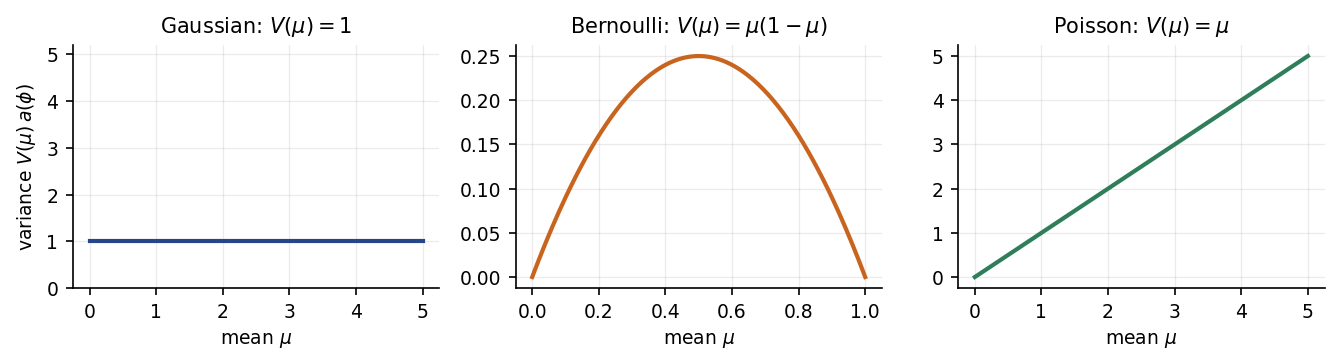
\includegraphics[width=0.92\textwidth,height=0.52\textheight,keepaspectratio]{adv04_varfun.png}
  \end{center}
  \begin{takeaway}
    Gaussian: flat variance, whatever the mean. Bernoulli: variance peaks at $0.25$
    when $\mu=0.5$ and vanishes at the ends. Poisson: variance climbs one-for-one with
    the mean --- at $\mu=5$ the variance \emph{must} be $5$. Data that violate the chosen
    line (as \texttt{Bikeshare} will, spectacularly) violate the family.
  \end{takeaway}
\end{frame}

% ------------------------------------------------------------
\begin{frame}{Exercise A4.2 --- The Bernoulli as a family member [Math]}
\begin{exercise}
  Let $Y\in\{0,1\}$ with $P(Y=1)=\mu$, so $f(y;\mu) = \mu^{y}(1-\mu)^{1-y}$.
  \begin{enumerate}
    \item Rewrite $f$ in exponential-family form and identify $\theta(\mu)$, $b(\theta)$
          and $a(\phi)$.
    \item Verify $b'(\theta) = \mu$.
    \item Verify $b''(\theta) = \mu(1-\mu)$, and state in one sentence what this
          variance function implies for observations with $\mu$ near $0.5$ versus near
          $0.99$.
  \end{enumerate}
\end{exercise}
\end{frame}

\begin{frame}{Solution --- Exercise A4.2}
\begin{solutionbox}
  \textbf{Method.} Take logs, isolate the coefficient of $y$, and match term by term.

  \textbf{Part 1.}
  $\log f = y\log\mu + (1-y)\log(1-\mu)
          = y\log\frac{\mu}{1-\mu} + \log(1-\mu)$, hence
  \[
    \theta = \log\frac{\mu}{1-\mu} \;\;(\text{the \textbf{logit}}), \qquad
    a(\phi)=1, \qquad c(y,\phi)=0 .
  \]
  Inverting the logit gives $\mu = e^{\theta}/(1+e^{\theta})$, so
  $\log(1-\mu) = -\log(1+e^{\theta})$ and therefore
  $b(\theta) = \log(1+e^{\theta})$.

  \textbf{Part 2.} $b'(\theta) = \dfrac{e^{\theta}}{1+e^{\theta}} = \mu$ \checkmark ---
  the sigmoid of Chapter 4.

  \textbf{Part 3.} $b''(\theta) = \dfrac{e^{\theta}}{(1+e^{\theta})^2}
  = \mu(1-\mu)$ \checkmark. Near $\mu=0.5$ the variance is maximal ($0.25$): most
  informative about $\beta$; near $\mu = 0.99$ it is $0.0099$ --- nearly
  deterministic, little information.
\end{solutionbox}
\begin{mistake}
  $b(\theta)$ must be written \textbf{as a function of $\theta$}, not of $\mu$ ---
  differentiating $b = -\log(1-\mu)$ with respect to $\theta$ as if $\mu$ were
  constant gives nonsense.
\end{mistake}
\end{frame}

% ============================================================
\section{GLM Anatomy}
% ============================================================

\begin{frame}{The three components of a GLM}
  \footnotesize
  \begin{block}{Rule (GLM specification)}
    \footnotesize
    \textbf{1.\ Random component:} $Y_i$ exponential-family with mean $\mu_i$.\quad
    \textbf{2.\ Systematic component:} linear predictor
    $\eta_i = \beta_0 + \beta_1 x_{i1} + \dots + \beta_p x_{ip}$.\quad
    \textbf{3.\ Link:} $\;\boxed{\,g(\mu_i) \;=\; \eta_i \;=\; x_i^{\top}\beta\,}$
  \end{block}
  \begin{readme}
    \begin{itemize}
      \item The link $g$ maps the mean's natural range onto the whole real line, where
            a linear predictor can roam freely: $\log:(0,\infty)\to\mathbb{R}$,
            $\text{logit}:(0,1)\to\mathbb{R}$.
      \item The \textbf{canonical link} sets $g = (b')^{-1}$, i.e.\ $\theta_i = \eta_i$:
            identity for Gaussian, logit for Bernoulli, log for Poisson --- concave
            log-likelihoods, simple score equations.
      \item Estimation is by \textbf{maximum likelihood}, via iteratively reweighted
            least squares (IRLS --- sketch in the appendix).
    \end{itemize}
  \end{readme}
  \begin{takeaway}
    Chapter 3 $=$ Gaussian $+$ identity. Chapter 4 $=$ Bernoulli $+$ logit. Today's
    workhorse $=$ Poisson $+$ log. Same anatomy, three organs swapped.
  \end{takeaway}
\end{frame}

\begin{frame}{Logistic regression, re-derived in one line}
  \footnotesize
  \begin{numexample}[Chapter 4 falls out as a special case]
    Take the Bernoulli member ($\theta=\log\frac{\mu}{1-\mu}$) and impose the
    canonical link $\theta_i = \eta_i$:
    \[
      \log\frac{p(x_i)}{1-p(x_i)} = \beta_0 + \beta_1 x_{i1} + \dots + \beta_p x_{ip}
      \quad\Longleftrightarrow\quad
      p(x_i) = \frac{e^{x_i^{\top}\beta}}{1+e^{x_i^{\top}\beta}} .
    \]
    This \emph{is} equation (4.6) of ISLP --- and ``$e^{\beta_j}$ multiplies the
    odds'' is the Bernoulli twin of the rate ratios two slides ahead.
  \end{numexample}
  \begin{takeaway}
    Nothing about logistic regression was ad hoc: sigmoid, log-odds reading, ML
    fitting --- all forced by ``Bernoulli $+$ canonical link''.
  \end{takeaway}
  \begin{industry}[Credit scoring: the regulated GLM]
    Default models in banking are Bernoulli GLMs: every $e^{\beta_j}$ has a
    documented odds-ratio meaning --- a key reason GLMs survive in the
    deep-learning era.
  \end{industry}
\end{frame}

\begin{frame}{Poisson regression: the model for \texttt{Bikeshare}}
  \begin{block}{Rule (Poisson GLM with log link)}
    \[
      Y_i \sim \text{Poisson}(\mu_i), \qquad
      \log \mu_i = \beta_0 + \beta_1 x_{i1} + \dots + \beta_p x_{ip}
      \;\;\Longleftrightarrow\;\;
      \mu_i = e^{\beta_0}\, e^{\beta_1 x_{i1}} \cdots e^{\beta_p x_{ip}} .
    \]
  \end{block}
  \begin{readme}[The multiplicative reading]
    \begin{itemize}
      \item $\mu_i > 0$ automatically --- no negative bikers, ever.
      \item One unit of $x_j$, rest fixed: the expected count is \emph{multiplied} by
            $e^{\beta_j}$ --- the \textbf{rate ratio} ($>1$ more bikers, $<1$ fewer).
      \item The variance follows along: $\operatorname{Var}(Y_i)=\mu_i$ --- busy hours
            are automatically noisier.
    \end{itemize}
  \end{readme}
  \begin{takeaway}
    Coefficients act on the \textbf{log of the mean}; effects on the count scale are
    \textbf{multiplicative}, never additive.
  \end{takeaway}
\end{frame}

\begin{frame}[fragile]{Fitting it in \texttt{statsmodels}}
\begin{lstlisting}
import numpy as np, pandas as pd
import statsmodels.api as sm, statsmodels.formula.api as smf

bike = pd.read_csv('Bikeshare.csv', index_col=0)     # 8 645 hourly rows
bike['hr'] = bike['hr'].astype(int)                  # hour 0..23
form = 'bikers ~ C(hr) + temp + workingday + C(weathersit)'
pois = smf.glm(form, data=bike,
               family=sm.families.Poisson()).fit()   # log link = canonical
print(pois.deviance, pois.df_resid)                  # 269 006 on 8 616 df
print(np.exp(pois.params['temp']))                   # rate ratio 4.79
\end{lstlisting}
  \begin{labnote}
    Notebook \texttt{advanced\_04\_glms\_splines\_lab.ipynb}, \S 3 \emph{Poisson
    regression on Bikeshare}: runs this fit, prints the full summary table and
    reproduces every rate ratio quoted on the next slide.
  \end{labnote}
\end{frame}

\begin{frame}{Reading the fitted coefficients as rate ratios}
  \footnotesize
  \begin{center}
  \begin{tabular}{@{}lrrr@{}}
    \toprule
    \textbf{Term} & $\hat\beta$ & SE & $e^{\hat\beta}$ (rate ratio) \\
    \midrule
    Intercept & $3.042$ & $0.009$ & $20.9$ bikers (baseline hour) \\
    \texttt{temp} & $1.567$ & $0.005$ & $4.79$ per full unit of temp \\
    \texttt{workingday} & $0.002$ & $0.002$ & $1.002$ \\
    \texttt{weathersit=cloudy/misty} & $-0.051$ & $0.002$ & $0.951$ \\
    \texttt{weathersit=light rain/snow} & $-0.505$ & $0.004$ & $0.603$ \\
    \texttt{weathersit=heavy rain/snow} & $-1.349$ & $0.167$ & $0.260$ \;(!) --- from $n=1$ hour \\
    \texttt{hr=8} \,/\, \texttt{hr=17} \,/\, \texttt{hr=4} & $1.826$ / $1.970$ / $-2.045$ & & $6.21$ / $7.17$ / $0.129$ vs midnight \\
    \bottomrule
  \end{tabular}
  \end{center}
  \begin{numexample}[Three concrete readings]
    \begin{itemize}
      \item \textbf{Light rain} cuts the expected count to $e^{-0.505}=0.603$ of the
            clear-sky rate --- \textbf{39.7\% fewer riders}, all else equal.
      \item $+0.1$ \texttt{temp} ($\approx 4^{\circ}$C) multiplies the rate by
            $e^{0.1\times 1.567} = 1.17$ --- \textbf{$+$17\% riders}.
      \item Rush hour vs night: $e^{\,1.970-(-2.045)} = e^{4.015} = \mathbf{55.4}$ ---
            17:00 carries $55\times$ the 04:00 rate.
    \end{itemize}
  \end{numexample}
  \begin{takeaway}
    Report $e^{\hat\beta}$, not $\hat\beta$ --- and distrust coefficients built on one
    observation (heavy rain).
  \end{takeaway}
\end{frame}

\begin{frame}{Offsets: modelling rates when exposure varies}
  \footnotesize
  \begin{block}{Rule (offset)}
    \footnotesize
    If $Y_i$ is a count accumulated over exposure $t_i$ (hours open, policy-years,
    population), model the \emph{rate} $\mu_i/t_i$:
    \quad $\log\dfrac{\mu_i}{t_i} = x_i^{\top}\beta
      \;\Longleftrightarrow\;
      \log\mu_i = \underbrace{\log t_i}_{\text{offset: coefficient fixed at }1} +\; x_i^{\top}\beta$.
  \end{block}
  \begin{numexample}[Why raw counts mislead]
    Station A: $30$ rentals in $2$ hours $\Rightarrow 15.0$/hour. Station B: $60$
    rentals in $6$ hours $\Rightarrow 10.0$/hour. B has \emph{twice} A's count but
    only $\tfrac{2}{3}$ of its rate; the offset makes the GLM compare $15.0$ vs
    $10.0$ --- the comparison you actually want.
  \end{numexample}
  \begin{takeaway}
    An offset is a covariate with $\beta$ \textbf{frozen at 1}:
    \texttt{smf.glm(..., offset=np.log(t))}. (\texttt{Bikeshare} needs none ---
    every row is exactly one hour.)
  \end{takeaway}
  \begin{industry}[Insurance and epidemiology: the offset is the law of the land]
    Claim counts per policy-year and disease counts per $100\,000$ population are
    \emph{always} fitted with exposure offsets --- otherwise big portfolios and big
    cities dominate for size alone.
  \end{industry}
\end{frame}

% ------------------------------------------------------------
\begin{frame}{Exercise A4.3 --- Rate ratios on \texttt{Bikeshare} [Python]}
\begin{exercise}
  Using the fitted Poisson GLM
  (\texttt{bikers $\sim$ C(hr) + temp + workingday + C(weathersit)}):
  \begin{enumerate}
    \item Compute the rate ratio for \texttt{light rain/snow} versus \texttt{clear},
          and phrase it as a percentage change in expected riders.
    \item The \texttt{temp} coefficient is $\hat\beta = 1.567$. By what factor does the
          expected count change when \texttt{temp} rises by $0.2$ (about
          $8^{\circ}$C)? Write the one line of Python that computes it from
          \texttt{pois.params}.
    \item Why would it be wrong to say ``a $0.2$ rise in temp \emph{adds}
          $0.2\times 1.567 = 0.31$ bikers''?
  \end{enumerate}
\end{exercise}
\begin{labnote}
  The worked solution sits in \texttt{advanced\_04\_glms\_splines\_lab.ipynb} under
  \emph{Lecture exercises --- worked Python solutions}: the cell headed
  \emph{Exercise A4.3 --- Rate ratios on Bikeshare}.
\end{labnote}
\end{frame}

\begin{frame}{Solution --- Exercise A4.3}
\begin{solutionbox}
  \textbf{Method.} All effects live on the log-mean scale; exponentiate to get
  multiplicative effects on the count scale.

  \textbf{Part 1.} $\hat\beta_{\text{light rain}} = -0.505$, so the rate ratio is
  $e^{-0.505} = 0.603$: light rain/snow is associated with
  $1-0.603 = \mathbf{39.7\%}$ \emph{fewer} expected riders than clear weather, holding
  hour, temperature and day type fixed.

  \textbf{Part 2.} Factor $= e^{0.2\times 1.567} = e^{0.313} = \mathbf{1.368}$ ---
  about $+36.8\%$.
  \begin{center}\ttfamily float(np.exp(0.2 * pois.params['temp']))\ \ \#\ 1.368\end{center}

  \textbf{Part 3.} $0.31$ is a change in $\log\mu$, not in $\mu$. The additive reading
  confuses the two scales: the actual change in expected riders depends on the starting
  level --- $+36.8\%$ of $10$ riders is $\approx 3.7$ riders, of $400$ riders
  $\approx 147$. Multiplicative effects have no single additive equivalent.
\end{solutionbox}
\begin{mistake}
  Treating GLM coefficients like OLS slopes. On the log link, $\hat\beta_j$ is a
  \textbf{log rate ratio}; only $e^{\hat\beta_j}$ has a direct count-scale meaning.
\end{mistake}
\end{frame}

% ============================================================
\section{Inference}
% ============================================================

\begin{frame}{Deviance: the GLM's residual sum of squares}
  \footnotesize
  \begin{block}{Rule (deviance)}
    \footnotesize
    With $\hat\ell_{\text{sat}}$ the log-likelihood of the \emph{saturated} model
    (one parameter per observation, each $y_i$ fitted exactly):
    \[
      D \;=\; 2\,\big(\hat\ell_{\text{sat}} - \hat\ell\,\big)
      \qquad\text{(}\phi = 1\text{; Poisson: } D = 2\textstyle\sum_i\big[\,y_i\log\tfrac{y_i}{\hat\mu_i} - (y_i-\hat\mu_i)\big]\text{)}.
    \]
  \end{block}
  \begin{readme}
    \begin{itemize}
      \item Smaller $D$ $=$ closer to a perfect fit; for the Gaussian, $D$ \emph{is}
            the RSS --- deviance generalises Chapter 3.
      \item The \textbf{null deviance} $D_0$ (intercept-only model) plays the role of
            the total sum of squares.
      \item \texttt{Bikeshare}: $D_0 = 1\,052\,921$ on $8\,644$ df
            $\to D = 269\,006$ on $8\,616$ df --- the $28$ predictors remove
            $\sim\!74\%$ of the null deviance.
    \end{itemize}
  \end{readme}
  \begin{takeaway}
    Deviance is to GLMs what RSS is to OLS: the currency in which fits are compared.
  \end{takeaway}
\end{frame}

\begin{frame}{Likelihood-ratio tests: comparing nested GLMs}
  \footnotesize
  \begin{block}{Rule (LRT)}
    \footnotesize
    For nested models (reduced $\subset$ full, differing by $q$ parameters), under
    $H_0$ ``the extra parameters are zero'':
    \[
      \text{LR} \;=\; D_{\text{reduced}} - D_{\text{full}}
      \;=\; 2\,(\hat\ell_{\text{full}} - \hat\ell_{\text{reduced}})
      \;\;\overset{H_0}{\sim}\;\; \chi^2_{q} \quad (n\to\infty).
    \]
  \end{block}
  \begin{numexample}[Does weather matter once hour + temp + day type are in?]
    Drop \texttt{weathersit} ($q = 3$ dummies):
    $D_{\text{reduced}} = 287\,263$, $D_{\text{full}} = 269\,006$, so
    $\text{LR} = 18\,256.8$ on $3$ df against a $5\%$ critical value of
    $\chi^2_{3,0.95} = 7.81$; $p$ is numerically $0$. Weather stays in.
  \end{numexample}
  \begin{takeaway}
    The GLM analogue of Chapter 3's $F$-test for a group of coefficients --- same
    logic, $\chi^2$ instead of $F$.
  \end{takeaway}
  \begin{mistake}
    The $\chi^2$ result needs \emph{nested} models fitted to the \emph{same rows} by
    \emph{maximum likelihood} --- it does not apply to quasi-likelihood fits.
  \end{mistake}
\end{frame}

\begin{frame}{AIC: model selection beyond nesting (bridge to Ch.\ 6)}
  \footnotesize
  \begin{block}{Rule (Akaike information criterion)}
    \footnotesize
    $\text{AIC} = -2\hat\ell + 2p$ \quad (smaller is better; $p$ $=$ number of parameters).
  \end{block}
  \begin{numexample}[On \texttt{Bikeshare}]
    Full Poisson model: $\hat\ell = -161\,022$, $p = 29 \Rightarrow \text{AIC} =
    322\,102$. Without \texttt{weathersit}: $\text{AIC} = 340\,352$. The full model
    wins by $18\,251$ AIC points --- consistent with the LRT.
  \end{numexample}
  \begin{readme}
    \begin{itemize}
      \item Chapter 6's AIC for regression was the Gaussian special case of this one.
      \item AIC compares \textbf{non-nested} models too (Poisson-with-splines vs
            Poisson-with-dummies) --- as long as both are true likelihoods
            \emph{for the same response data}.
    \end{itemize}
  \end{readme}
  \begin{takeaway}
    Deviance for nested tests, AIC for menus of candidates --- both are likelihood
    arithmetic, both carry over to GAMs.
  \end{takeaway}
\end{frame}

% ------------------------------------------------------------
\begin{frame}{Exercise A4.4 --- Deviance, LRT and AIC by hand [Math]}
\begin{exercise}
  For the \texttt{Bikeshare} Poisson GLM you are given:
  full model $D = 269\,005.9$ on $8\,616$ df, $\hat\ell = -161\,021.8$, $p = 29$;
  reduced model (no \texttt{weathersit}) $D = 287\,262.7$, $p = 26$.
  \begin{enumerate}
    \item Compute the likelihood-ratio statistic for \texttt{weathersit} and its
          degrees of freedom.
    \item Compare with $\chi^2_{3,0.95} = 7.81$ and state the conclusion.
    \item Compute the full model's AIC from $\hat\ell$ and $p$.
    \item The reduced model's AIC is $340\,352.4$. Recover its log-likelihood.
  \end{enumerate}
\end{exercise}
\end{frame}

\begin{frame}{Solution --- Exercise A4.4}
\begin{solutionbox}
  \textbf{Method.} Deviance differences are likelihood-ratio statistics; AIC is
  $-2\hat\ell + 2p$ --- everything is plug-in arithmetic.

  \textbf{Part 1.} $\text{LR} = D_{\text{red}} - D_{\text{full}}
  = 287\,262.7 - 269\,005.9 = \mathbf{18\,256.8}$, with
  $q = 29 - 26 = \mathbf{3}$ df (three weather dummies).

  \textbf{Part 2.} $18\,256.8 \gg 7.81$: reject $H_0$ decisively --- weather adds
  explanatory power far beyond chance, given hour, temperature and day type.

  \textbf{Part 3.} $\text{AIC} = -2(-161\,021.8) + 2\times 29
  = 322\,043.7 + 58.0 = \mathbf{322\,101.7}$ \checkmark (matches
  \texttt{statsmodels}).

  \textbf{Part 4.} $\hat\ell_{\text{red}} = -(\text{AIC} - 2p)/2
  = -(340\,352.4 - 52)/2 = \mathbf{-170\,150.2}$. Check:
  $2(\hat\ell_{\text{full}} - \hat\ell_{\text{red}})
  = 2(-161\,021.8 + 170\,150.2) = 18\,256.8$ \checkmark --- the same LR as Part 1.
\end{solutionbox}
\begin{mistake}
  Comparing AICs of models fitted to \textbf{different responses} (e.g.\ $y$ vs
  $\log y$) or different subsets of rows. AIC differences are only meaningful on
  identical data.
\end{mistake}
\end{frame}

% ============================================================
\section{Overdispersion}
% ============================================================

\begin{frame}{The Poisson straitjacket: variance $=$ mean, no exceptions}
  The Poisson family has \textbf{no free variance parameter}: choosing it \emph{asserts}
  $\operatorname{Var}(Y_i) = \mu_i$.
  \begin{numexample}[\texttt{Bikeshare} violates this on every shelf]
    Group the hours into cells of (hour $\times$ day type $\times$ weather), keep the
    $119$ cells with $n\ge 20$:
    \begin{itemize}
      \item 5\,p.m., working day, clear: mean $431.5$, variance $23\,085$ ---
            ratio $\mathbf{53.5}$.
      \item 4\,a.m., working day, clear: mean $4.97$, variance $7.4$ --- ratio $1.5$.
      \item \textbf{All 119 cells} have variance above their mean; the median ratio is
            $\mathbf{27.7}$.
    \end{itemize}
  \end{numexample}
  \begin{takeaway}
    Counts in the wild are almost always \textbf{overdispersed}: unmodelled
    heterogeneity (events, marketing, school holidays\ldots) inflates the variance
    beyond Poisson. The mean model can still be fine --- the \emph{uncertainty} is not.
  \end{takeaway}
\end{frame}

\begin{frame}{Seeing the violation: variance vs mean across cells}
  \begin{center}
    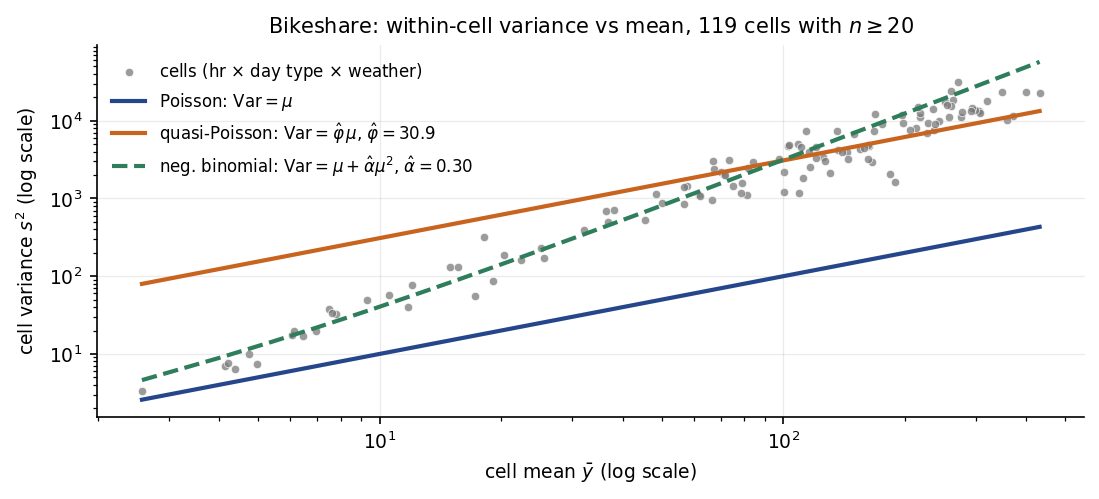
\includegraphics[width=0.88\textwidth,height=0.56\textheight,keepaspectratio]{adv04_meanvar.png}
  \end{center}
  \begin{takeaway}
    The Poisson line $\operatorname{Var}=\mu$ runs far below every cell. The
    quasi-Poisson line $\hat\varphi\,\mu$ with $\hat\varphi = 30.9$ matches mid-range
    cells; the negative-binomial curve $\mu + 0.30\,\mu^2$ bends up to catch the busy,
    high-variance cells. The data choose the curved law.
  \end{takeaway}
\end{frame}

\begin{frame}{Fix 1 --- quasi-Poisson: rescale the uncertainty}
  \begin{block}{Rule (quasi-likelihood with dispersion)}
    Keep the mean model and $V(\mu)=\mu$, but allow
    $\operatorname{Var}(Y_i) = \varphi\,\mu_i$, estimating
    \[
      \hat\varphi \;=\; \frac{X^2}{n-p} \;=\; \frac{1}{n-p}\sum_{i=1}^{n}\frac{(y_i-\hat\mu_i)^2}{\hat\mu_i},
      \qquad
      \widehat{\text{SE}}_{\text{quasi}}(\hat\beta_j) = \sqrt{\hat\varphi}\;\widehat{\text{SE}}_{\text{Pois}}(\hat\beta_j).
    \]
  \end{block}
  \begin{numexample}[\texttt{Bikeshare}]
    $X^2 = 266\,229$ on $n-p = 8\,616$ df $\Rightarrow \hat\varphi = \mathbf{30.90}$:
    every standard error grows by $\sqrt{30.90} = \mathbf{5.56}$.
    \textbf{Point estimates do not move.} Consequences:
    \texttt{temp} $z$: $330 \to 59.4$ (still overwhelming);
    \texttt{workingday} $z$: $1.19 \to \mathbf{0.21}$ --- its apparent effect
    evaporates.
  \end{numexample}
  \begin{takeaway}
    Overdispersion rarely changes \emph{what} the effects are --- it changes
    \emph{how sure you are}. Borderline stars are the first casualties.
  \end{takeaway}
\end{frame}

\begin{frame}{Fix 2 --- negative binomial: model the extra variance}
  \footnotesize
  \begin{block}{Rule (NB2 negative binomial)}
    \footnotesize
    Let $Y_i \mid G_i \sim \text{Poisson}(\mu_i G_i)$ with a gamma-distributed
    multiplicative effect $G_i$ ($E[G_i]=1$, $\operatorname{Var}(G_i)=\alpha$). Then
    \;$E[Y_i] = \mu_i$, \quad $\operatorname{Var}(Y_i) = \mu_i + \alpha\,\mu_i^2$.
  \end{block}
  \begin{numexample}[\texttt{Bikeshare}]
    ML estimate $\hat\alpha = \mathbf{0.305}$. Log-likelihood improves from
    $-161\,022$ (Poisson) to $-45\,266$ (NB); AIC drops from $322\,102$ to
    $\mathbf{90\,590}$ --- not a close call. At $\mu = 400$ the implied variance is
    $400 + 0.305\times 400^2 \approx 49\,200$, versus Poisson's $400$.
  \end{numexample}
  \begin{readme}[Quasi vs NB in one line each]
    \emph{Quasi-Poisson}: same estimates, honest SEs, \textbf{no likelihood} (no AIC,
    no LRT). \emph{Negative binomial}: a genuine likelihood --- estimates shift (it
    reweights observations), AIC/LRT available, variance grows \emph{quadratically}.
  \end{readme}
  \begin{takeaway}
    Only need honest standard errors? Quasi suffices. Need likelihood machinery or
    predictive distributions? Fit the negative binomial.
  \end{takeaway}
\end{frame}

\begin{frame}{Poisson vs quasi-Poisson vs negative binomial, side by side}
  \footnotesize
  \begin{center}
  \begin{tabular}{@{}lrrrrr@{}}
    \toprule
    & \multicolumn{2}{c}{\textbf{Poisson}} & \textbf{quasi-Poisson} & \multicolumn{2}{c}{\textbf{Negative binomial}} \\
    \cmidrule(lr){2-3}\cmidrule(lr){4-4}\cmidrule(lr){5-6}
    \textbf{Term} & $\hat\beta$ & SE & SE ($\times 5.56$) & $\hat\beta$ & SE \\
    \midrule
    \texttt{temp} & $1.567$ & $0.005$ & $0.026$ & $1.894$ & $0.032$ \\
    \texttt{workingday} & $0.002$ & $0.002$ & $0.011$ & $-0.195$ & $0.013$ \\
    \texttt{light rain/snow} & $-0.505$ & $0.004$ & $0.022$ & $-0.538$ & $0.022$ \\
    \midrule
    AIC & \multicolumn{2}{c}{$322\,102$} & --- (no likelihood) & \multicolumn{2}{c}{$90\,590$} \\
    \bottomrule
  \end{tabular}
  \end{center}
  \begin{readme}[Which numbers changed --- and why]
    Quasi keeps every $\hat\beta$ and multiplies SEs by $\sqrt{\hat\varphi}=5.56$. NB
    \emph{refits}: its likelihood downweights huge counts, so estimates move ---
    \texttt{workingday} even flips sign, because its true effect is heterogeneous
    across hours (positive at commuter peaks, negative at night) and the two
    likelihoods average that heterogeneity with different weights.
  \end{readme}
  \begin{industry}[Retail demand: the dispersion audit]
    Demand-forecasting teams sanity-check $\hat\varphi$ per store cluster. A jump of
    $\hat\varphi$ from 3 to 30 after a promotion week is a red flag that the mean model
    is missing a driver --- not a licence for tighter intervals.
  \end{industry}
\end{frame}

% ------------------------------------------------------------
\begin{frame}{Exercise A4.5 --- Dispersion arithmetic [Math]}
\begin{exercise}
  The \texttt{Bikeshare} Poisson fit has Pearson statistic $X^2 = 266\,229$ with
  $n = 8\,645$ observations and $p = 29$ parameters. The \texttt{temp} coefficient is
  $\hat\beta = 1.567$ with Poisson SE $0.0047$.
  \begin{enumerate}
    \item Estimate the dispersion $\hat\varphi$ and the factor by which all standard
          errors must grow.
    \item Compute the 95\% confidence interval for $\beta_{\texttt{temp}}$ under the
          Poisson fit and under quasi-Poisson (use $\pm 1.96\,\text{SE}$).
    \item Convert both intervals to rate-ratio scale.
    \item A colleague argues: ``the quasi interval is wider, so the Poisson one is more
          precise --- keep it.'' Rebut in one sentence.
  \end{enumerate}
\end{exercise}
\end{frame}

\begin{frame}{Solution --- Exercise A4.5}
\begin{solutionbox}
  \textbf{Method.} $\hat\varphi = X^2/(n-p)$; quasi SEs scale by $\sqrt{\hat\varphi}$;
  exponentiate CI endpoints for rate ratios.

  \textbf{Part 1.} $\hat\varphi = 266\,229 / (8\,645 - 29) = 266\,229/8\,616 =
  \mathbf{30.90}$; SEs grow by $\sqrt{30.90} = \mathbf{5.56}$.

  \textbf{Part 2.} Poisson: $1.567 \pm 1.96 \times 0.0047 = [\,1.558,\; 1.576\,]$.
  Quasi: SE $= 5.56\times 0.0047 = 0.0264$, so
  $1.567 \pm 1.96\times 0.0264 = [\,1.515,\; 1.619\,]$.

  \textbf{Part 3.} Rate-ratio scale: Poisson $[\,e^{1.558}, e^{1.576}\,] =
  [\,4.75,\; 4.83\,]$; quasi $[\,e^{1.515}, e^{1.619}\,] = [\,4.55,\; 5.05\,]$.

  \textbf{Part 4.} The Poisson interval is not \emph{more precise}, it is
  \emph{wrong}: its claimed coverage assumes $\operatorname{Var}=\mu$, which the data
  contradict by a factor of $\sim\!31$, so the narrow interval covers the truth far
  less often than 95\%.
\end{solutionbox}
\begin{mistake}
  Reading interval width as a quality metric. Width is only meaningful \emph{after} the
  variance assumption survives a check like $\hat\varphi \approx 1$.
\end{mistake}
\end{frame}

% ------------------------------------------------------------
\begin{frame}{Extended Exercise A4.1 --- The overdispersion pipeline [Integrative]}
\begin{longexercise}[Extended exercise (15 min) --- from suspicion to model choice]
  Work through the full overdispersion protocol on \texttt{Bikeshare}
  (\texttt{bikers $\sim$ C(hr) + temp + workingday + C(weathersit)}):
  \begin{enumerate}
    \item \textbf{Diagnose.} Compute $\hat\varphi$ from the Poisson fit's Pearson
          statistic. What values would have let you keep plain Poisson?
    \item \textbf{Repair the SEs.} Which of the following change under quasi-Poisson,
          and how: point estimates, standard errors, fitted means, AIC?
    \item \textbf{Re-model.} The negative binomial fit gives $\hat\alpha = 0.305$ and
          AIC $90\,590$ vs Poisson's $322\,102$. Why is comparing these two AICs
          legitimate, while ``quasi-Poisson AIC'' does not exist?
    \item \textbf{Decide.} \texttt{workingday} has $\hat\beta = 0.002$ (Poisson),
          $z_{\text{quasi}} = 0.21$, but $\hat\beta = -0.195$ (NB, $z \approx -14.7$).
          What should an analyst conclude and report about the working-day effect?
  \end{enumerate}
\end{longexercise}
\begin{labnote}
  Notebook \S 5 \emph{Overdispersion: quasi-Poisson and negative binomial} fits all
  three models and prints the comparison table from the previous slide.
\end{labnote}
\end{frame}

\begin{frame}{Solution --- Extended Exercise A4.1 (1/2)}
\begin{solutionbox}[Solution --- diagnosis and repair]
  \textbf{Method.} One dispersion statistic drives the whole protocol; then separate
  what quasi-likelihood rescales from what a new likelihood refits.

  \textbf{Part 1.} $\hat\varphi = 266\,229/8\,616 = 30.90$. Values near $1$
  (rule of thumb $\lesssim 1.5$, given the huge $n$ here even tighter) would justify
  plain Poisson; $30.9$ is a categorical rejection --- the variance is
  $\sim\!31\times$ the Poisson claim on average.

  \textbf{Part 2.} Under quasi-Poisson: point estimates \textbf{unchanged} (same
  estimating equations); fitted means \textbf{unchanged}; standard errors
  \textbf{multiplied by} $\sqrt{30.90}=5.56$; AIC \textbf{undefined} ---
  quasi-likelihood is not a likelihood, so there is no $\hat\ell$ to plug into
  $-2\hat\ell + 2p$.
\end{solutionbox}
\end{frame}

\begin{frame}{Solution --- Extended Exercise A4.1 (2/2)}
\begin{solutionbox}[Solution --- re-model and decide]
  \textbf{Part 3.} Poisson and negative binomial are both \emph{genuine likelihoods
  for the same response vector}, so their AICs are comparable: the NB's
  $90\,590 \ll 322\,102$ says the quadratic variance law fits these counts far
  better. Quasi-Poisson specifies only mean and variance, never a density, hence
  no likelihood and no AIC.

  \textbf{Part 4.} The honest conclusion: \emph{averaged over all hours}, working days
  do not add a stable multiplicative effect --- quasi says the average effect is
  indistinguishable from zero, and the NB's $-0.195$ reflects its different weighting
  of hours, not a newly discovered negative effect. The effect is
  \textbf{heterogeneous} (strongly positive at 8\,a.m.\ and 5--6\,p.m., negative at
  night and midday); report it via an \emph{interaction} (workingday $\times$ hour) or
  a GAM with separate hour curves, not a single number.
\end{solutionbox}
\begin{mistake}
  Reading the sign flip as ``the NB found the true effect''. When two reasonable
  likelihoods disagree this much, the model is mis-specified --- the fix is a richer
  mean model, not a coin flip between packages.
\end{mistake}
\end{frame}

% ============================================================
\section{Penalized Splines}
% ============================================================

\begin{frame}{Chapter 7 recap: regression splines and the knot dilemma}
  \begin{readme}[What you already know]
    \begin{itemize}
      \item A \textbf{regression spline} of degree 3 is a piecewise cubic, forced to be
            continuous with continuous first and second derivatives at the \textbf{knots}.
      \item Fit by OLS on a spline \textbf{basis}: flexibility is controlled by the
            \emph{number and placement of knots} (equivalently, the degrees of freedom).
      \item Chapter 7's recipe: place knots at quantiles, pick df by cross-validation.
    \end{itemize}
  \end{readme}
  \begin{takeaway}[The dilemma this section resolves]
    Knot choice is \textbf{discrete and awkward}: 5 vs 6 knots is a lumpy, all-or-nothing
    decision, and knots in the wrong place cannot be undone by fitting. The penalized
    view replaces ``how many knots?'' by a single \textbf{continuous} dial $\lambda$:
    use \emph{plenty} of knots, then penalise wiggliness.
  \end{takeaway}
\end{frame}

\begin{frame}{The B-spline basis: local, overlapping bumps}
  \begin{center}
    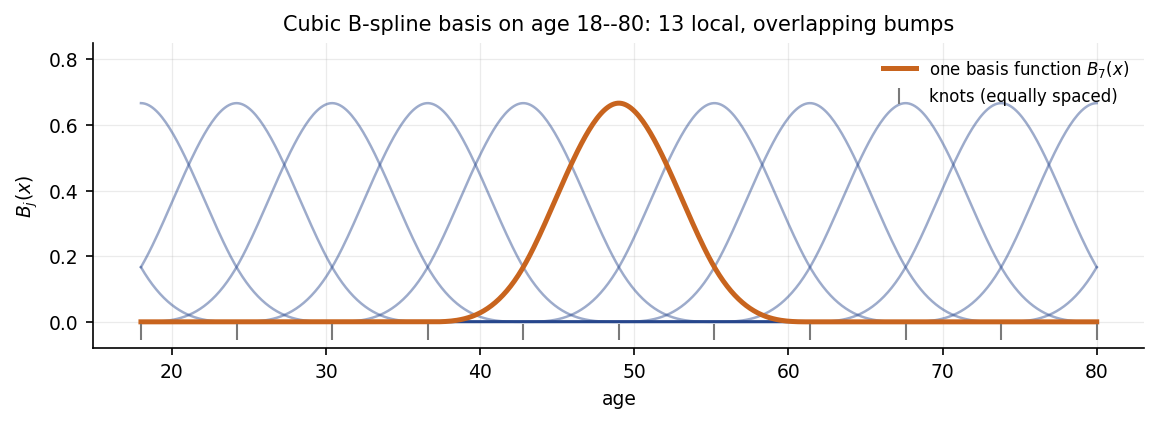
\includegraphics[width=0.9\textwidth,height=0.5\textheight,keepaspectratio]{adv04_bspline_basis.png}
  \end{center}
  \begin{takeaway}
    Each cubic B-spline $B_j(x)$ is positive on only $4$ adjacent knot intervals and
    zero elsewhere; at any $x$ they sum to $1$. The fit
    $f(x)=\sum_j \beta_j B_j(x)$ is a \textbf{local} blend --- moving one $\beta_j$
    reshapes the curve only near its bump, which is why the basis is numerically
    stable where raw polynomials ($x^7$, $x^8$, \dots) explode.
  \end{takeaway}
\end{frame}

\begin{frame}{Penalized splines: many knots, one dial}
  \footnotesize
  \begin{block}{Rule (penalized fitting)}
    \footnotesize
    Use a rich B-spline basis ($20$--$40$ knots) and minimise
    \[
      \boxed{\;\underbrace{\text{Deviance}(\beta)}_{\text{fit the data}}
      \;+\; \lambda \underbrace{\int f''(t)^2\, dt}_{\text{punish wiggliness}}\;}
      \qquad\text{with } \int f''(t)^2 dt = \beta^{\top} S \beta .
    \]
    Gaussian case: $\hat\beta_\lambda = (B^{\top}B + \lambda S)^{-1} B^{\top} y$ ---
    ridge regression (Ch.\ 6) with a structured penalty.
  \end{block}
  \begin{readme}
    $\lambda = 0$: unpenalized --- as wiggly as the basis allows.
    \;$\lambda \to \infty$: $f''\equiv 0$ forced --- a \textbf{straight line} (zero
    curvature is invisible to the penalty).
    \;In between: the bias--variance dial of Chapter 2, turned \emph{continuously}.
  \end{readme}
  \begin{takeaway}
    Knot placement stops mattering once knots are plentiful; \textbf{all} structural
    choice is concentrated in the single number $\lambda$.
  \end{takeaway}
\end{frame}

\begin{frame}{Effective degrees of freedom: how much did you really fit?}
  \footnotesize
  \begin{block}{Rule (edf)}
    \footnotesize
    The penalized fit is linear in $y$: $\hat y = H(\lambda)\, y$ with smoother matrix
    $H(\lambda) = B\,(B^{\top}B + \lambda S)^{-1} B^{\top}$. Define
    \[
      \text{edf}(\lambda) \;=\; \operatorname{tr}\{H(\lambda)\}
      \;=\; \sum_{k} \frac{1}{1 + \lambda d_k},
      \qquad d_k \ge 0 \text{ the penalty's eigenvalues in the basis.}
    \]
  \end{block}
  \begin{numexample}[Toy computation]
    Four basis directions with $d = (0,\, 0,\, 1,\, 4)$ and $\lambda = 1$:
    $\text{edf} = 1 + 1 + \tfrac{1}{2} + \tfrac{1}{5} = \mathbf{2.7}$. The two $d=0$
    directions (constant, linear --- zero curvature) are never shrunk; the wiggly ones
    are partially switched off.
  \end{numexample}
  \begin{takeaway}
    edf interpolates smoothly between $2$ (a line) and $K$ (the full basis) --- ``this
    smooth is worth $6.3$ parameters'' is a meaningful, comparable statement.
  \end{takeaway}
\end{frame}

\begin{frame}{Choosing $\lambda$: cross-validation or GCV (bridge to Ch.\ 5)}
  \footnotesize
  \begin{block}{Rule (generalized cross-validation)}
    \footnotesize
    \[
      \text{GCV}(\lambda) \;=\; \frac{n\,\text{RSS}(\lambda)}{\big(n - \text{edf}(\lambda)\big)^{2}}
      \qquad\text{--- minimise over } \lambda .
    \]
  \end{block}
  \begin{readme}
    \begin{itemize}
      \item GCV is a shortcut to leave-one-out CV: no $n$ refits, just the single fit's
            edf --- the same idea as Chapter 5's LOOCV formula for linear smoothers.
      \item $k$-fold CV on a $\lambda$-grid works too --- the honest default when the
            model is not a linear smoother (e.g.\ GLM deviance losses).
      \item Watch \textbf{edf}, not $\lambda$: $\lambda$'s scale depends on the basis,
            edf does not.
    \end{itemize}
  \end{readme}
  \begin{takeaway}
    $\lambda$ is a tuning parameter like any in Chapters 5--6: chosen by (generalized)
    cross-validation, never by eye.
  \end{takeaway}
\end{frame}

\begin{frame}{One picture: \texttt{Wage} across three orders of magnitude of $\lambda$}
  \begin{center}
    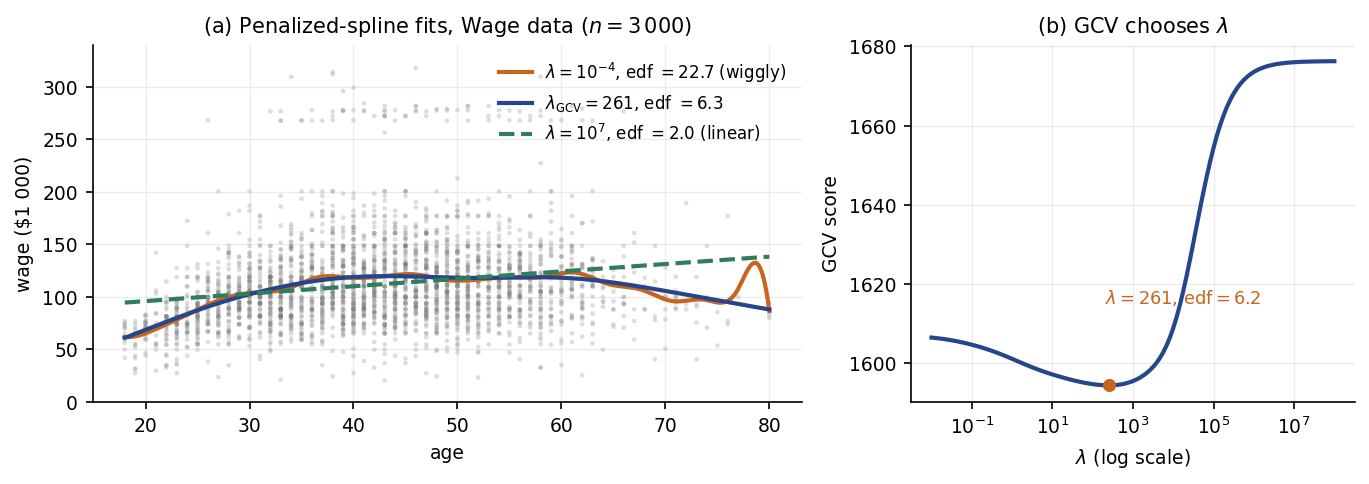
\includegraphics[width=0.95\textwidth,height=0.56\textheight,keepaspectratio]{adv04_pspline_lambda.png}
  \end{center}
  \begin{takeaway}
    $23$ cubic B-splines on \texttt{age} ($n = 3\,000$). At $\lambda=10^{-4}$ the fit
    burns $22.7$ edf and chases noise around age 78; at $\lambda=10^{7}$ it collapses
    to a line ($2.0$ edf) and misses the plateau. GCV picks
    $\lambda = 261$, $\text{edf} = 6.3$ --- close to the df Chapter 7 found by CV for
    this very curve.
  \end{takeaway}
\end{frame}

% ------------------------------------------------------------
\begin{frame}{Exercise A4.6 --- Reading the $\lambda$ dial [Math]}
\begin{exercise}
  A penalized cubic spline uses $K = 23$ B-spline basis functions with a
  second-derivative penalty $S$ whose null space contains exactly the constant and
  linear functions.
  \begin{enumerate}
    \item State $\text{edf}$ in the limits $\lambda \to 0$ and $\lambda \to \infty$,
          with one sentence of justification each.
    \item In a small example the penalty eigenvalues are $d = (0, 0, 1, 4)$. Compute
          $\text{edf}$ for $\lambda = 1$ and for $\lambda = 4$.
    \item Your colleague reports ``$\lambda = 261$'' as the headline of their smooth.
          Why is ``$\text{edf} = 6.3$'' the better headline?
  \end{enumerate}
\end{exercise}
\end{frame}

\begin{frame}{Solution --- Exercise A4.6}
\begin{solutionbox}
  \textbf{Method.} Use $\text{edf}(\lambda) = \sum_k 1/(1+\lambda d_k)$ and think about
  which directions the penalty can and cannot touch.

  \textbf{Part 1.} $\lambda \to 0$: no shrinkage, every basis direction survives,
  $\text{edf} \to K = \mathbf{23}$ (an unpenalized regression spline).
  $\lambda \to \infty$: every direction with $d_k > 0$ is annihilated; only the
  null space of $S$ --- constant $+$ linear --- survives, so
  $\text{edf} \to \mathbf{2}$ (a straight line).

  \textbf{Part 2.} $\lambda = 1$:
  $1 + 1 + \tfrac{1}{1+1} + \tfrac{1}{1+4} = 2 + 0.5 + 0.2 = \mathbf{2.70}$.\\
  $\lambda = 4$:
  $1 + 1 + \tfrac{1}{5} + \tfrac{1}{17} = 2 + 0.200 + 0.059 = \mathbf{2.26}$ ---
  quadrupling $\lambda$ removed less than half an edf: the dial is logarithmic.

  \textbf{Part 3.} $\lambda$'s numerical value depends on the basis size, the knot
  spacing, even the units of $x$ --- $261$ is meaningless across studies. edf is
  invariant to all of that and reads directly as model complexity:
  ``a curve worth $6.3$ parameters''.
\end{solutionbox}
\begin{mistake}
  Comparing $\lambda$ values across different bases or datasets. Only \textbf{edf}
  travels.
\end{mistake}
\end{frame}

% ============================================================
\section{GAMs for Counts}
% ============================================================

\begin{frame}{The meeting point: GAM $=$ GLM $+$ smooth terms}
  \begin{block}{Rule (penalized-spline GAM for counts)}
    \[
      Y_i \sim \text{Poisson}(\mu_i), \qquad
      \log \mu_i \;=\; \beta_0 \;+\; f_1(\texttt{hr}_i) \;+\; f_2(\texttt{temp}_i)
      \;+\; \beta_w\,\texttt{workingday}_i \;+\; \textstyle\sum_k \gamma_k\, \texttt{weather}_{ik},
    \]
    each $f_j$ a penalized B-spline with its own $\lambda_j$; fit by
    \textbf{penalized maximum likelihood} (penalized IRLS).
  \end{block}
  \begin{readme}
    \begin{itemize}
      \item Everything from this module composes: exponential family (random part),
            log link, deviance-based fitting, roughness penalties per smooth.
      \item Chapter 7 introduced GAMs with fixed-df smoothers; the upgrade here is that
            each curve's complexity is \emph{estimated} via $\lambda_j$, not preset.
      \item Additivity is retained: each $f_j$ is a one-dimensional curve you can
            \emph{plot and defend} --- the interpretability contract of Ch.\ 7 survives.
    \end{itemize}
  \end{readme}
  \begin{takeaway}
    A GAM for counts answers the module's opening problem in full: positive means,
    variance tied to the mean, and no guessed functional forms.
  \end{takeaway}
\end{frame}

\begin{frame}[fragile]{Fitting the GAM with \texttt{statsmodels}}
\begin{lstlisting}
from statsmodels.gam.api import GLMGam, BSplines

xs = bike[['hr', 'temp']].astype(float)
bs = BSplines(xs, df=[12, 6], degree=[3, 3])       # rich bases for hr, temp
Xpar = ...   # intercept, workingday, 3 weather dummies (parametric part)

gam = GLMGam(bike.bikers, exog=Xpar, smoother=bs,
             family=sm.families.Poisson(), alpha=[0.319, 0.00423])
res = gam.fit()
# the two penalty weights above were chosen by the built-in criterion:
#   gam.select_penweight()[0]   ->  [0.319, 0.00423]
print(res.deviance)                                 # 259 650
\end{lstlisting}
  \begin{labnote}
    Notebook \S 7 \emph{A penalized-spline GAM for Bikeshare} builds \texttt{Xpar},
    runs \texttt{select\_penweight}, and draws the partial-effect plots on the next
    slide with confidence bands.
  \end{labnote}
\end{frame}

\begin{frame}{What the machine chose}
  \begin{numexample}[Selected penalties and complexity on \texttt{Bikeshare}]
    \begin{itemize}
      \item \texttt{select\_penweight} (GCV-type criterion) returns
            $\hat\alpha = (0.319,\; 0.00423)$ for (\texttt{hr}, \texttt{temp}).
      \item Resulting complexity: hour smooth $\approx \mathbf{11}$ edf, temperature
            smooth $\approx \mathbf{5}$ edf --- the light penalties keep almost all of
            the $12$ and $6$ basis df: with $8\,645$ observations the data can afford it.
      \item Deviance $259\,650$ vs $269\,006$ for the dummy-\texttt{hr} GLM with linear
            \texttt{temp}; AIC $312\,730$ vs $322\,102$ --- the smooth-temp model wins
            by $\sim\!9\,400$ AIC points with \emph{fewer} effective parameters.
    \end{itemize}
  \end{numexample}
  \begin{takeaway}
    The gain comes almost entirely from letting \texttt{temp} \textbf{bend}: the
    linear-temp assumption of the earlier GLM was the binding constraint, not the
    hour dummies.
  \end{takeaway}
\end{frame}

\begin{frame}{The fitted smooths: hour of day and temperature}
  \begin{center}
    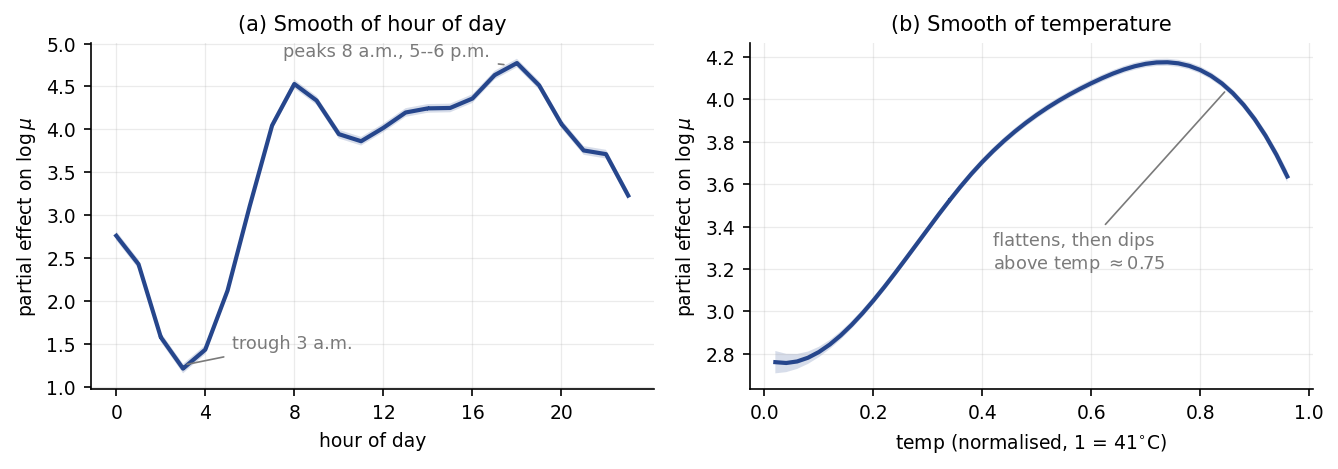
\includegraphics[width=0.92\textwidth,height=0.56\textheight,keepaspectratio]{adv04_gam_partial.png}
  \end{center}
  \begin{takeaway}
    \textbf{Hour}: trough at 3\,a.m., twin commuter peaks at 8\,a.m.\ and 5--6\,p.m.;
    peak-to-trough ratio $e^{4.77-1.21} = \mathbf{35\times}$. \textbf{Temp}: riders
    triple ($\times 3.1$) from temp $0.2$ to $0.7$, then \emph{fall} beyond
    $\approx 0.75$ ($\sim 31^{\circ}$C) --- a hot-weather dip a linear term is
    structurally unable to show.
  \end{takeaway}
\end{frame}

\begin{frame}{Interpreting the hour curve --- and one honest caveat}
  \begin{readme}[Reading a partial effect]
    Each curve shows the contribution to $\log\mu$ \emph{holding the other terms
    fixed}. Differences along one curve exponentiate to rate ratios:
    $f(18) - f(3) = 4.77 - 1.21 = 3.56 \Rightarrow e^{3.56} \approx 35\times$ more
    riders at 6\,p.m.\ than at 3\,a.m., same weather, same temperature, same day type.
  \end{readme}
  \begin{mistake}[Smooths smooth --- also where the truth is spiky]
    The dummy model rates 17:00 at $\mathbf{55.4\times}$ the 04:00 level; the smooth
    version says $24.6\times$. The penalty shrinks the razor-sharp night dip and
    commuter spikes toward their neighbours. For genuinely \emph{discontinuous}
    patterns (timetables, opening hours), factors or more basis df beat a heavily
    penalized smooth --- check edf and residuals by hour before trusting the curve.
  \end{mistake}
  \begin{industry}[Energy: GAMs run the grid]
    European system operators forecast national electricity load with exactly this
    structure --- smooth(hour), smooth(temperature), calendar dummies --- because
    engineers must \emph{see and sign off} each curve. The hot-weather bend
    (air conditioning) is the industry's textbook example of why temp must be a smooth.
  \end{industry}
\end{frame}

\begin{frame}{Pitfalls when GLMs meet splines}
  \begin{alertblock}{Don't}
    \begin{enumerate}
      \item \textbf{Extrapolate a spline.} Outside the knot range the fit continues as
            a low-order polynomial with \emph{no data behind it}; on the log scale a
            mild linear overshoot exponentiates into absurd counts.
      \item \textbf{Read smooths causally.} $f(\texttt{temp})$ is an association given
            the other terms; hot hours also differ in season, daylight and tourism.
            Nothing here is a do-operator.
      \item \textbf{Ignore overdispersion because the mean is now flexible.} The GAM's
            deviance is still Poisson: with $\hat\varphi \approx 31$ on this data, its
            naive confidence bands are $\sim\!5.6\times$ too narrow too. Rescale or go NB.
    \end{enumerate}
  \end{alertblock}
  \begin{takeaway}
    Flexibility fixes the \emph{mean}; it does not buy causality and it does not fix
    the \emph{variance}. Keep the three audits separate.
  \end{takeaway}
\end{frame}

% ------------------------------------------------------------
\begin{frame}{Extended Exercise A4.2 --- Build and defend a count GAM [Python]}
\begin{longexercise}[Extended exercise (15 min) --- the full modelling arc]
  Using \texttt{GLMGam} with \texttt{BSplines(df=[12, 6], degree=[3, 3])} on
  \texttt{hr} and \texttt{temp}, plus parametric \texttt{workingday} and weather
  dummies:
  \begin{enumerate}
    \item Write down the model equation for $\log\mu_i$ and say which parts are
          penalized.
    \item The selected penalties give edf $\approx 11$ (hr) and $\approx 5$ (temp).
          What would edf $\approx 2$ for \texttt{temp} have told you?
    \item From the fitted hour smooth, $f(18) = 4.77$ and $f(3) = 1.21$. Compute the
          6\,p.m.\ vs 3\,a.m.\ rate ratio and interpret it in one sentence.
    \item The GAM's weather coefficient is $-0.569$ (light rain) vs the GLM's
          $-0.505$. Give one reason the estimates differ.
    \item Name the single most important robustness check before this model ships to
          the fleet-rebalancing team.
  \end{enumerate}
\end{longexercise}
\begin{labnote}
  Notebook \S 7 closes with this exercise: the cell headed \emph{Extended Exercise
  A4.2} reproduces every number.
\end{labnote}
\end{frame}

\begin{frame}{Solution --- Extended Exercise A4.2 (1/2)}
\begin{solutionbox}[Solution --- model / edf / rate ratio]
  \textbf{Method.} Assemble the GAM equation, then read complexity from edf and
  effects from differences on the log scale.

  \textbf{Part 1.}
  $\log\mu_i = \beta_0 + f_1(\texttt{hr}_i) + f_2(\texttt{temp}_i)
  + \beta_w \texttt{workingday}_i + \gamma_1\texttt{cloudy}_i
  + \gamma_2\texttt{light}_i + \gamma_3\texttt{heavy}_i$.
  Only $f_1$ and $f_2$ are penalized (each with its own $\alpha$); intercept, dummies
  and $\beta_w$ are ordinary ML parameters.

  \textbf{Part 2.} edf $\approx 2$ for \texttt{temp} would mean the penalty had shrunk
  the smooth to (near-)linearity --- i.e.\ the data see no curvature and the Ch.\ 4
  linear-temp GLM would have been adequate. The actual edf $\approx 5$ says the bend
  (including the hot-weather dip) is real structure worth $\sim\!5$ parameters.

  \textbf{Part 3.} $e^{\,4.77 - 1.21} = e^{3.56} \approx \mathbf{35}$: holding
  temperature, weather and day type fixed, the expected count at 6\,p.m.\ is about
  $35$ times the 3\,a.m.\ count.
\end{solutionbox}
\end{frame}

\begin{frame}{Solution --- Extended Exercise A4.2 (2/2)}
\begin{solutionbox}[Solution --- coefficient shift and the shipping check]
  \textbf{Part 4.} The two models adjust for temperature differently: the GLM forces a
  linear \texttt{temp} effect, the GAM lets it bend. Rainy hours are also cool hours,
  so when the temperature adjustment changes shape, the weather dummies absorb a
  different share of the rain--cold overlap ($-0.569$ vs $-0.505$). Coefficients of
  correlated regressors always move when a co-regressor's functional form changes.

  \textbf{Part 5.} An \textbf{overdispersion audit} of the GAM itself: compute the
  Pearson dispersion of the GAM fit (it remains $\gg 1$ on this data) and widen the
  uncertainty accordingly (quasi rescaling or an NB-GAM). Shipping the $35\times$
  headline with Poisson bands would overstate certainty roughly $5$--$6$-fold ---
  the fleet team would over-trust hour-level differences that are partly noise.
\end{solutionbox}
\begin{mistake}
  Declaring victory after the mean model improves. The variance audit
  (\S Overdispersion) applies to GAMs verbatim --- flexible means do not repair
  broken variances.
\end{mistake}
\end{frame}

% ============================================================
\section{Summary}
% ============================================================

\begin{frame}{Module A4 in one slide}
  \begin{block}{What we accomplished}
    \begin{itemize}
      \item Diagnosed why OLS fails on counts: negative means, constant variance ---
            $10\%$ negative predictions on \texttt{Bikeshare}.
      \item Unified Chs.\ 3--4 in the \textbf{exponential family}: mean $b'(\theta)$,
            variance $b''(\theta) a(\phi)$.
      \item Assembled the \textbf{GLM}: family $+$ linear predictor $+$ link; Poisson
            coefficients as \textbf{rate ratios}; offsets for exposure.
      \item Ran GLM \textbf{inference}: deviance, LRT ($18\,257$ on $3$ df for weather),
            AIC.
      \item Confronted \textbf{overdispersion} ($\hat\varphi = 30.9$): quasi-Poisson
            rescales SEs $\times 5.56$; negative binomial ($\hat\alpha = 0.305$) refits.
      \item Rebuilt splines as \textbf{penalized} fits: one dial $\lambda$, complexity
            read as edf, tuned by GCV/CV.
      \item Met in the middle: a \textbf{penalized-spline Poisson GAM} with
            interpretable hour and temperature curves.
    \end{itemize}
  \end{block}
\end{frame}

\begin{frame}{Key formulas at a glance}
  \footnotesize
  \begin{description}
    \item[Exponential family] $f(y;\theta,\phi) = \exp\{(y\theta - b(\theta))/a(\phi) + c(y,\phi)\}$
    \item[Mean and variance] $E[Y] = b'(\theta)$, \quad $\operatorname{Var}(Y) = b''(\theta)\,a(\phi) = a(\phi)V(\mu)$
    \item[GLM link] $g(\mu_i) = \eta_i = x_i^{\top}\beta$; canonical link $g = (b')^{-1}$
    \item[Poisson rate ratio] one unit of $x_j$ multiplies $\mu$ by $e^{\beta_j}$; offset: $\log\mu_i = \log t_i + x_i^{\top}\beta$
    \item[Deviance / LRT] $D = 2(\hat\ell_{\text{sat}} - \hat\ell)$; \quad $D_{\text{red}} - D_{\text{full}} \sim \chi^2_q$ under $H_0$
    \item[AIC] $-2\hat\ell + 2p$
    \item[Dispersion] $\hat\varphi = X^2/(n-p)$; quasi SE $= \sqrt{\hat\varphi}\,\times$ Poisson SE
    \item[Negative binomial] $\operatorname{Var}(Y) = \mu + \alpha\mu^2$
    \item[Penalized spline] minimise $\text{Deviance} + \lambda \int f''(t)^2 dt = \text{Dev} + \lambda\,\beta^{\top}S\beta$
    \item[Effective df] $\text{edf} = \operatorname{tr}\{B(B^{\top}B+\lambda S)^{-1}B^{\top}\} = \sum_k (1+\lambda d_k)^{-1}$
    \item[GCV] $n\,\text{RSS}/(n-\text{edf})^2$
    \item[Count GAM] $\log\mu_i = \beta_0 + \sum_j f_j(x_{ij}) + (\text{parametric terms})$
  \end{description}
\end{frame}

\begin{frame}{Vocabulary checklist}
  \footnotesize
  \begin{center}
  \begin{tabular}{@{}ll@{}}
    \toprule
    \textbf{Term} & \textbf{Meaning} \\
    \midrule
    Canonical parameter $\theta$ & natural scale on which $y$ enters the density linearly \\
    Cumulant function $b(\theta)$ & generates mean ($b'$) and variance ($b''$) \\
    Variance function $V(\mu)$ & mandated shape of variance as a function of the mean \\
    Link function $g$ & maps the mean's range to $\mathbb{R}$; canonical if $g=(b')^{-1}$ \\
    Linear predictor $\eta$ & $x^{\top}\beta$, the part shared with Chs.\ 3--4 \\
    Rate ratio & $e^{\beta_j}$: multiplicative effect on the expected count \\
    Offset & covariate with coefficient fixed at 1, encodes exposure \\
    Saturated model / deviance & perfect-fit benchmark; $2\times$ log-likelihood gap to it \\
    Overdispersion & $\operatorname{Var} > $ family's claim; here $\hat\varphi = 30.9$ \\
    Quasi-likelihood & mean--variance assumptions only; no density, no AIC \\
    Negative binomial & gamma-mixed Poisson; $\operatorname{Var}=\mu+\alpha\mu^2$ \\
    B-spline basis & local overlapping polynomial bumps; numerically stable \\
    Roughness penalty & $\lambda\int f''^2$: price tag on curvature \\
    Effective df (edf) & $\operatorname{tr}\,H(\lambda)$: parameters actually spent \\
    GCV & leave-one-out shortcut for linear smoothers \\
    GAM / partial effect & additive smooth terms inside a GLM; one curve per predictor \\
    \bottomrule
  \end{tabular}
  \end{center}
\end{frame}

\begin{frame}{Decision rules of thumb}
  \begin{itemize}
    \item Response is a \textbf{count} $\Rightarrow$ start with Poisson $+$ log link;
          \textbf{binary} $\Rightarrow$ Bernoulli $+$ logit; \textbf{continuous
          symmetric} $\Rightarrow$ Gaussian $+$ identity.
    \item Counts accumulated over unequal windows $\Rightarrow$ \textbf{offset}
          $\log(\text{exposure})$, always.
    \item After any Poisson fit, compute $\hat\varphi = X^2/(n-p)$. If
          $\hat\varphi \gtrsim 1.5$: quasi-Poisson for quick honest SEs; negative
          binomial when you need AIC, LRTs or predictive distributions.
    \item Effect shape unknown $\Rightarrow$ penalized spline with generous basis;
          let GCV/CV set $\lambda$; \textbf{report edf}, not $\lambda$.
    \item Smooth's edf $\approx 2$ $\Rightarrow$ simplify to a linear term; edf near the
          basis size $\Rightarrow$ consider a larger basis or a factor.
    \item Report $e^{\hat\beta}$ (rate/odds ratios) with intervals from the
          \emph{dispersion-corrected} fit.
  \end{itemize}
  \begin{takeaway}
    Family first, link second, dispersion audit third, smoothness by CV fourth ---
    in that order, every time.
  \end{takeaway}
\end{frame}

\begin{frame}{Common pitfalls}
  \begin{alertblock}{Don't}
    \begin{enumerate}
      \item \textbf{Fit OLS to raw counts} (or to $\log(y+1)$ and call it equivalent) ---
            wrong support, wrong variance, biased back-transformed means.
      \item \textbf{Interpret GLM coefficients additively} --- on a log link only
            $e^{\hat\beta}$ speaks the count language.
      \item \textbf{Trust Poisson standard errors without a dispersion check} --- at
            $\hat\varphi = 30.9$ they are $5.6\times$ too small; borderline
            ``discoveries'' evaporate.
      \item \textbf{Use AIC/LRT on quasi-likelihood fits} --- there is no likelihood
            there.
      \item \textbf{Extrapolate splines beyond the knots} or compare raw $\lambda$
            values across bases --- use edf and stay in range.
      \item \textbf{Read GAM smooths as causal effects} --- they are adjusted
            associations, nothing more.
    \end{enumerate}
  \end{alertblock}
\end{frame}

\begin{frame}{Self-check questions}
  \begin{readme}[Can you answer these without the slides?]
    \begin{enumerate}
      \item Derive the mean and variance of the Poisson from $b(\theta) = e^{\theta}$.
      \item Why is the logit the \emph{canonical} link for the Bernoulli, and what
            does canonicality buy?
      \item Weather's LRT was $18\,257$ on $3$ df. Which two models were compared, and
            what assumption makes the $\chi^2$ reference valid?
      \item Quasi-Poisson and negative binomial both ``fix'' overdispersion --- name
            two practical situations that force the NB choice.
      \item Why does $\lambda\to\infty$ leave a straight line rather than a constant,
            for a second-derivative penalty?
      \item Your GAM's temperature smooth has edf $5.0$ and dips after temp $0.75$.
            What would you check before presenting the dip as real?
    \end{enumerate}
  \end{readme}
  \begin{takeaway}
    If question 1 takes more than two lines, revisit the worked Poisson derivation ---
    it is the single most exam-relevant computation of this module.
  \end{takeaway}
\end{frame}

% ============================================================
\appendix
\AtBeginSection[]{}
\section{Appendix: optional and advanced material}
% ============================================================

\begin{frame}{Appendix --- what is in here, and why}
  Nothing in the appendix is needed to follow the chapter: each slide is a formal
  derivation, a longer worked exercise, or a side topic. Read it when you want the
  full story, or when a later chapter sends you back here.
  \begin{block}{Contents of the appendix}
    \begin{itemize}
      \item \textbf{Score identities} --- the two-line proof of $E[Y]=b'(\theta)$ and
            $\operatorname{Var}(Y)=b''(\theta)a(\phi)$; moved out because the main deck
            only needs the result.
      \item \textbf{The Gaussian as a family member} --- completes the table of three;
            moved out because it mirrors the Poisson derivation done live.
      \item \textbf{IRLS in one slide} --- how GLMs are actually fitted; moved out
            because no lecture decision depends on the algorithm's internals.
      \item \textbf{Deviance formulas per family} --- reference table; moved out
            because it is look-up material, not narrative.
      \item \textbf{Drill exercise on offsets} --- extra practice with full solution;
            moved out to keep the main flow at two extended exercises.
    \end{itemize}
  \end{block}
\end{frame}

\begin{frame}{Score identities: where mean and variance come from}
  \footnotesize
  For one observation, $\ell(\theta) = \dfrac{y\theta - b(\theta)}{a(\phi)} + c(y,\phi)$.
  \begin{block}{Derivation}
    \emph{First identity.} Under regularity, $E\!\left[\partial\ell/\partial\theta\right] = 0$:
    \[
      E\!\left[\frac{Y - b'(\theta)}{a(\phi)}\right] = 0
      \;\;\Longrightarrow\;\; E[Y] = b'(\theta).
    \]
    \emph{Second identity.} The Bartlett identity
    $E\!\left[\partial^2\ell/\partial\theta^2\right]
     + E\!\left[(\partial\ell/\partial\theta)^2\right] = 0$ gives
    \[
      -\frac{b''(\theta)}{a(\phi)} + \frac{\operatorname{Var}(Y)}{a(\phi)^2} = 0
      \;\;\Longrightarrow\;\; \operatorname{Var}(Y) = b''(\theta)\,a(\phi). \qquad\blacksquare
    \]
  \end{block}
  \begin{takeaway}
    Both facts used throughout the module are two lines of calculus on the score ---
    no distribution-specific work needed.
  \end{takeaway}
\end{frame}

\begin{frame}{The Gaussian as a family member (completing the table)}
  \begin{numexample}[Match the normal density to the family form]
    \[
      f(y;\mu,\sigma^2)
      = \exp\!\left\{ \frac{y\mu - \mu^2/2}{\sigma^2}
        \;-\; \frac{y^2}{2\sigma^2} \;-\; \tfrac12\log(2\pi\sigma^2) \right\}.
    \]
    Matching: $\theta = \mu$, \; $b(\theta) = \theta^2/2$, \; $a(\phi) = \sigma^2$, \;
    $c(y,\phi) = -y^2/(2\sigma^2) - \tfrac12\log(2\pi\sigma^2)$.
    Identities: $E[Y] = b'(\theta) = \theta = \mu$ \checkmark;\;
    $\operatorname{Var}(Y) = b''(\theta)a(\phi) = 1\cdot\sigma^2$ \checkmark.
  \end{numexample}
  \begin{takeaway}
    $b'' \equiv 1$: the Gaussian is the \emph{only} member whose variance ignores the
    mean --- exactly the property that made OLS fail on counts, and exactly why
    Chapter 3 never needed a variance function.
  \end{takeaway}
\end{frame}

\begin{frame}{IRLS: how a GLM is actually fitted}
  \footnotesize
  \begin{block}{Algorithm (iteratively reweighted least squares)}
    Repeat until convergence, starting from any sensible $\hat\mu^{(0)}$:
    \begin{enumerate}
      \item Working response: \;
            $z_i = \hat\eta_i + (y_i - \hat\mu_i)\, g'(\hat\mu_i)$.
      \item Working weights: \;
            $w_i = \big[\, g'(\hat\mu_i)^2\, V(\hat\mu_i)\, \big]^{-1}$.
      \item Update $\beta$ by weighted least squares of $z$ on $X$ with weights $w$;
            set $\hat\eta = X\hat\beta$, $\hat\mu = g^{-1}(\hat\eta)$.
    \end{enumerate}
  \end{block}
  \begin{readme}
    \begin{itemize}
      \item IRLS is Newton--Raphson with the expected information (Fisher scoring),
            rearranged as repeated WLS --- which is why GLM software is built on the
            Chapter 3 machinery.
      \item Penalized GAM fitting only changes step 3: WLS becomes \emph{penalized}
            WLS with $\lambda S$ added --- the ridge update from Chapter 6.
    \end{itemize}
  \end{readme}
  \begin{takeaway}
    A GLM is ``OLS in a loop''; a GAM is ``ridge in a loop''. Nothing beyond this
    course's toolbox.
  \end{takeaway}
\end{frame}

\begin{frame}{Deviance formulas per family (reference)}
  \footnotesize
  \begin{center}
  \begin{tabular}{@{}lll@{}}
    \toprule
    \textbf{Family} & \textbf{Unit deviance contribution $d_i$} & \textbf{Note} \\
    \midrule
    Gaussian & $(y_i - \hat\mu_i)^2$ & $D = $ RSS: Ch.\ 3 recovered \\
    Bernoulli & $-2\big[\,y_i\log\hat\mu_i + (1-y_i)\log(1-\hat\mu_i)\,\big]$ & $=$ the cross-entropy loss \\
    Poisson & $2\big[\,y_i\log(y_i/\hat\mu_i) - (y_i - \hat\mu_i)\,\big]$ & terms with $y_i=0$: $2\hat\mu_i$ \\
    Neg.\ binomial & $2\big[ y_i\log\frac{y_i}{\hat\mu_i} - (y_i + \tfrac1\alpha)\log\frac{1+\alpha y_i}{1+\alpha\hat\mu_i} \big]$ & reduces to Poisson as $\alpha\to 0$ \\
    \bottomrule
  \end{tabular}
  \end{center}
  \begin{readme}
    $D = \sum_i d_i$ in each case. Residual checks for GLMs use \emph{deviance
    residuals} $\operatorname{sign}(y_i - \hat\mu_i)\sqrt{d_i}$, which are the closest
    GLM analogue of the OLS residuals from Chapter 3.
  \end{readme}
\end{frame}

\begin{frame}{Drill Exercise A4.A --- Offsets in anger [Math]}
\begin{exercise}
  A city compares cycling at two counting stations using a Poisson GLM with log link.
  Station~1 recorded $y_1 = 180$ riders over $t_1 = 12$ hours; Station~2 recorded
  $y_2 = 96$ riders over $t_2 = 4$ hours.
  \begin{enumerate}
    \item Compute each station's empirical rate per hour.
    \item In the model $\log\mu_i = \log t_i + \beta_0 + \beta_1 \mathbb{1}\{i=2\}$,
          express $e^{\beta_1}$ in terms of the two rates and compute its ML estimate.
    \item What would the same model \emph{without} the offset (raw counts) have
          estimated for $e^{\beta_1}$, and why is that misleading?
  \end{enumerate}
\end{exercise}
\end{frame}

\begin{frame}{Solution --- Drill Exercise A4.A}
\begin{solutionbox}
  \textbf{Method.} With a saturated two-group Poisson model, ML fits each group's rate
  exactly --- so everything reduces to ratios of empirical rates.

  \textbf{Part 1.} Station 1: $180/12 = \mathbf{15.0}$ riders/hour.
  Station 2: $96/4 = \mathbf{24.0}$ riders/hour.

  \textbf{Part 2.} With the offset, $\mu_i = t_i\, e^{\beta_0 + \beta_1\mathbb{1}\{i=2\}}$,
  so $e^{\beta_0}$ is Station 1's rate and $e^{\beta_1}$ the \textbf{rate ratio}:
  \[
    e^{\hat\beta_1} = \frac{y_2/t_2}{y_1/t_1} = \frac{24.0}{15.0} = \mathbf{1.60}
  \]
  --- Station 2 sees $60\%$ \emph{more} riders per hour.

  \textbf{Part 3.} Without the offset the model compares raw counts:
  $e^{\hat\beta_1} = 96/180 = \mathbf{0.533}$ --- Station 2 would look $47\%$
  \emph{quieter}, purely because it was observed for a third of the time. Same data,
  opposite conclusion; the offset is what makes the comparison fair.
\end{solutionbox}
\begin{mistake}
  Adding exposure as an ordinary covariate ($\beta$ estimated) ``to be safe''. That
  lets the model bend the exposure effect away from proportionality and destroys the
  rate interpretation; the offset's whole point is $\beta_{\text{exposure}} \equiv 1$.
\end{mistake}
\end{frame}

\end{document}
